\chapter{Artificial Lattices}
\section{Introduction [not serious]}
Theoretical Physicist have been dreaming with theoretical models since they realized it was much easier to write down and solve some equations than find a material governed by such equations. For years without end, we have created more and more models, useful, and boring, and silly, and interesting ones, but just theoretical models non the less.

The problem of vacancies/adatoms in graphene has been widely studied, both theoretically and experimentally. On one hand, the experimental studies usually focus on the local properties of the localized states, lacking the capability to study ``complex'' structures of vacancies/adatoms. On the other hand, theoretical studies usually relay on calculations in which the translational symmetry of the crystal is preserved, what is generally considered a handicap for the model since experimentally the vacancies do not form an array large enough to behave as a crystal. Any effect derived from the consideration of a crystal of vacancies is usually neglected either as an artifact of the theory or an unachivable experimental option. If this limitation is avoided, then the theoretical study focus in single vacancies as experimental studies usually do.

Recent experimental advances have shown the capability to arrange large areas/quantities of atoms with atomic precision\cite{Brihuega2016,Kalff2016}.
An obvious question is whether or not we can build artificial lattices by placing adatoms on graphene.

The idea is to use a large flake of graphene bilayer (the reasons will be explored later in the text) in which the adatoms are placed in very specific atomic positions to form a (periodic) crystal. Since graphene can be described with a triangular or a rectangular Bravais lattice, many crystals are available by choosing the suitable unit cell and lattice vectors.


There are two main reasons to choose graphene bilayer as the platform to build artificial fermion models. The first one is that graphene (and by extension graphene bilayer) is the most studied material ever. The fabrication and tuning capabilities exceeds those of any other material. The second one is that its electronic properties are highly tunable whether it is via proximity to other materials or via the application of external fields.

% XXX move
% When an external electric field is applied to graphene bilayer, a tunable gap is open\cite{Zhang2009,Lui2011,Ponomarenko2011} (the maximum observed value is $\Delta_E\sim\SI{0.25}{\eV}$).


\section{General considerations} %~~~~~~~~~~~~~~~~~~~~~~~~~~~~~~~~~~~~~~~~~~~~~%
We are going to study the electronic states arose by vacancies in the $\pi$-manifold in graphene bilayer (GB) and its interactions with an external electric field, $V$.
We will consider isolated vacancies in order to study the properties of the electronic states. Later on, we will also study infinite periodic arrays of defects forming a crystal.\\

When only a finite number of vacancies are considered, the system used will be an armchair island, as such, the system is $0$-D, so there is no translational symmetry and no $\vec{k}$ vector can be defined, nor Bloch's theorem can be applied.

To study these systems we will consider a basis of localized states that could be considered to be the $p_z$ hydrogenoid orbitals.
\begin{equation}
  \mathcal{B} = \left\{\phi_1,\phi_2,\dots,\phi_\alpha,\dots,\phi_{N_C}\right\}
\end{equation}

The complete Hamiltonian will look like this:
\begin{equation}
  H = H_t + H_{t'} + H_{V}
\label{hamiltonian}
\end{equation}

The term $H_t$ represents the kinetic energy arising from the hopping between neighboring sites in the same layer, $H_{t'}$ represents the interlayer hoppings and the term $H_{V}$ corresponds to the effect of an external electric field on the electrons. Such a term is considered to be just a layer dependent shift in the on-site energies:
% \begin{equation}
%   H_{\lambda_E} = \lambda_E
%   \left(\begin{array}{cc}
%   \mathds{1} & 0 \\
%   0 & -\mathds{1}
%   \end{array}\right)
% \end{equation}
\begin{equation}
  H_{V} = V\lambda_l
\end{equation}
where $V$ is the potential difference between the two layers and $\lambda_l\in\{-1,1\}$ labels the layer.
The vacancies are introduced in this model as an infinite on-site energy for the chosen atom(s). Unless otherwise stated, everything is done in $eV$, \emph{not in hopping units}. The intralayer $p_z$-$p_z$ hopping is chosen as $t=\SI{-2.7}{\eV}$ and the interlayer $t'=\SI{0.4}{\eV}$ in accordance with the literature\cite{KatsnelsonBook}.\\

In the presence of vacancies, there will appear in-gap states (as many as vacancies are considered) which will be labeled by $\Psi_0$, $\Psi_1$, ... in order to distinguish them form any other eigenstate.
\begin{equation}
\begin{split}
  H\ket{\psi_\alpha} = E_\alpha\ket{\psi_\alpha} \qquad&;\qquad
\ket{\psi_\alpha} = \sum_\beta c_\beta\ket{\phi_\beta}\\
  H\ket{\Psi_0} &= E_0\ket{\Psi_0}
\end{split}
\end{equation}

%  \section{Effects of an external electric field}
%  
%  In order to open a gap in the band structure of graphene bilayer one has to apply an external electric field. One option would be to simply place an electric gate under the sample, but this approach will heavily charge the system as soon as free charges are available (for instance from a hypothetical source and drain contacts)\cite{McCann2006,Zhang2009,Taychatanapat2010}.
%  The other option is to use two gates, one on top of the sample and the other underneath it. Let us discuss the second option.
%  
%  
%  \subsection{Dual Gating}
%  Let us consider a graphene bilayer, depicted by the black lines and balls in Fig.~\ref{dual_gate}, sandwiched by $SiO_2$ layers and with two gates, unoriginally referred to as top and bottom, each with a voltage $V_{t/b}$ respectively. This setup will be consider as an infinite parallel plate capacitor.
%  %~~~~~~~~~~~~~~~~~~~~~~~~~~ FIGURE ~~~~~~~~~~~~~~~~~~~~~~~~~%
%  \begin{figure}[h!]
%  \centering
%  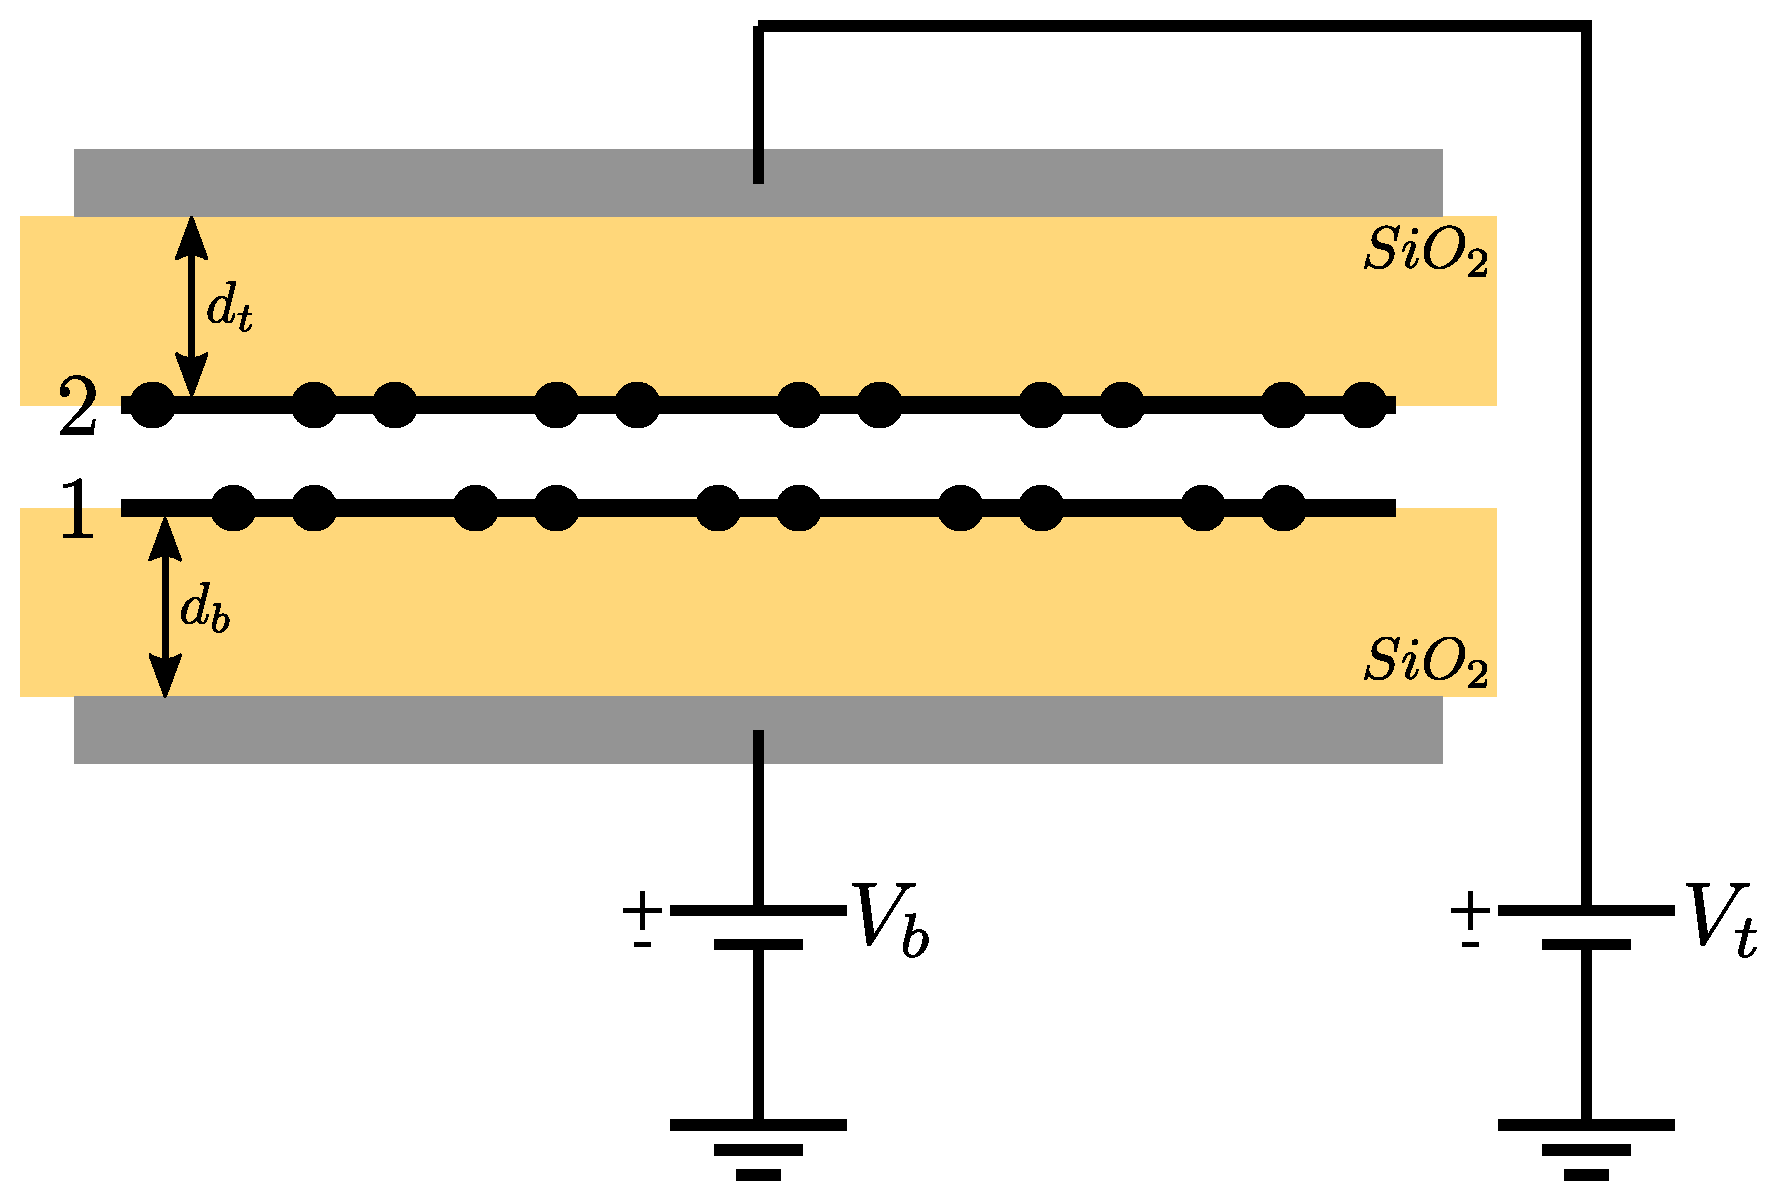
\includegraphics[width=0.5\textwidth]{artlat/fig/dual_gate.pdf}
%  \vspace{-5pt}
%  \caption{Schematics of dual gating.}
%  \label{dual_gate}
%  \end{figure}
%  \FloatBarrier
%  %~~~~~~~~~~~~~~~~~~~~~~~~~~~~~~~~~~~~~~~~~~~~~~~~~~~~~~~~~~~%
%  
%  The role of the electric field induced by the voltage $V_t$ and $V_b$ is twofold. On one hand, it will break the symmetry between the two layers by shifting their on-site energies, on the other hand it may dope the  system.
%  
%  The doping (extra charge absorbed into the system) in the graphene bilayer can be estimated simply by applying Gauss' law:
%  \begin{equation}
%     \diver{D} = \rho-\rho_0 = \rho_f
%  \label{gauss}
%  \end{equation}
%  where $\rho$ is total charge density, $\rho_0$ is the bounded charge density so that $\rho_f$ is the free charge density.
%  
%  Since we are considering an infinite capacitor, the electric field only has $z$ component, hence the divergence of the displacement results in a derivative which can be discretized:
%  \begin{equation}
%     \diver{D}=\frac{\partial D}{\partial z} =\frac{D_t-D_b}{dz} = \rho_f =
%     e\frac{N}{V} \Rightarrow D_t-D_b = e\delta n
%  \label{doping}
%  \end{equation}
%  where $N$ and $V=Adz$ are the number of electrons and volume ($A$ is the area), and $\delta n$ is the bidimensional density of electrons.
%  
%  In order to calculate the potential difference between the two graphene layers, we can consider simply the average of the electric field inside the capacitor:
%  \begin{equation}
%     \Delta V = \langle\vec{E}\rangle \Delta z = \frac{E_t+E_b}{2} \Delta z=
%     \frac{\Delta z}{2} \left(\frac{D_t}{\varepsilon_t} +
%                              \frac{D_b}{\varepsilon_b} \right)
%  \label{potential}
%  \end{equation}
%  where $\Delta z$ is width of the graphene bilayer and $\varepsilon_t$ and $\varepsilon_b$ are the electric permeability of the top and bottom dielectrics. $D_t$ and $D_b$ are (the $z$-component of) the displacement fields in the top and bottom regions.
%  \begin{equation}
%     D_t = \frac{\varepsilon_t}{d_t}\left(V_{t}-V^0_{t}\right) \qquad;\qquad
%     D_b = \frac{\varepsilon_b}{d_b}\left(V_{b}-V^0_{b}\right)
%  \end{equation}
%  where $V^0_{t/b}$ are the off-set potential required to have charge neutrality, usually referred to as \ac{cnp}.
%  
%  Equations \eqref{doping} and \eqref{potential} show that by choosing the appropriates $V_t$ and $V_b$ we can independently change the doping of the system and the gap opened in the band structure.
%  
%  
%  
%  \subsection{Hartree}
%  Using the basis $\mathcal{B}=\left\{\phi^1_A,\phi^1_B,\phi^2_A,                 \phi^2_B\right\}$ (where $A/B$ label sublattice and $1/2$ label the graphene    layer) we can write the basic Hamiltonian that models a graphene bilayer as:
%  \begin{equation}
%     H(\vec{k}) = \left(\begin{array}{cccc}
%           \epsilon_1 & f(\vec{k}) & 0 & 0 \\
%           f^*(\vec{k}) & \epsilon_1 & \gamma & 0 \\
%           0 & \gamma & \epsilon_2 & f(\vec{k}) \\
%           0 & 0 & f^*(\vec{k}) & \epsilon_2
%                  \end{array}\right)
%  \end{equation}
%  where $\epsilon_{1/2}$ account for both the shifting of the on-site energies  in each layer and the effect of having extra charge in the opposite layer.
%  \begin{equation}
%  \begin{split}
%     \epsilon_1 &= \frac{e}{\varepsilon_0}\Delta z \sigma_2 + V^0_1 \\
%     \epsilon_2 &= \frac{e}{\varepsilon_0}\Delta z \sigma_1 + V^0_2
%  \end{split}
%  \end{equation}
%  where $\sigma$ is the planar charge density, calculated as:
%  \begin{equation}
%     \sigma_{\text{bottom}} = \sum^{N_{\text{occ}}}_i |\bra{\psi_i}\mathcal{O}_B \ket{\psi_i}|^2
%     \frac{e}{N_k A}
%  \end{equation}
%  Each of the Hartree contributions, then will be:
%  \begin{equation}
%     \epsilon^{H}_1 = \frac{e^2\Delta z}{\varepsilon_0A}
%     \frac{1}{N_k}\sum|\mean{B}|^2
%  \end{equation}
%  The order of magnitude of the prefactor is:
%  \begin{equation}
%     \frac{e^2\Delta z}{\varepsilon_0A} =
%     \frac{\SI{2.56e-38}{\coulomb\squared} \cdot \SI{3.1e-10}{\meter}}
%     {\SI{8.8e-12}{\coulomb\per\volt\per\meter} \cdot \SI{5e-20}{\meter\squared}}=
%     \SI{1.75e-17}{\joule} \sim \SI{109.23}{\eV}
%  \end{equation}
%  where we have used that $\si{\joule}=\si{\coulomb\volt}$. The remaining factor $\tfrac{1}{Nk}\sum\langle B\rangle\sim 0.5$ since $|\mean{B}|^2\in[0,1]$
%  
%  
%  
%  The calculation of the first terms, has to be done iteratively since the estimation of electronic density, $\delta n$, depends on the eigenfunctions of the system, which depends on the on-site energies which depend on the electronic density.
%  
%  %
%  % XXX Calculate and describe the Hartree solution
%  %
%  
%  





\section{Biased bilayer graphene}
The electronic structure of bilayer graphene in the presence of an external electric field has been widely studied. Here I summarize the basic relevant properties.\\
%~~~~~~~~~~~~~~~~~~~~~~~~~~ FIGURE ~~~~~~~~~~~~~~~~~~~~~~~~~%
\begin{figure}[!ht!]
\centering
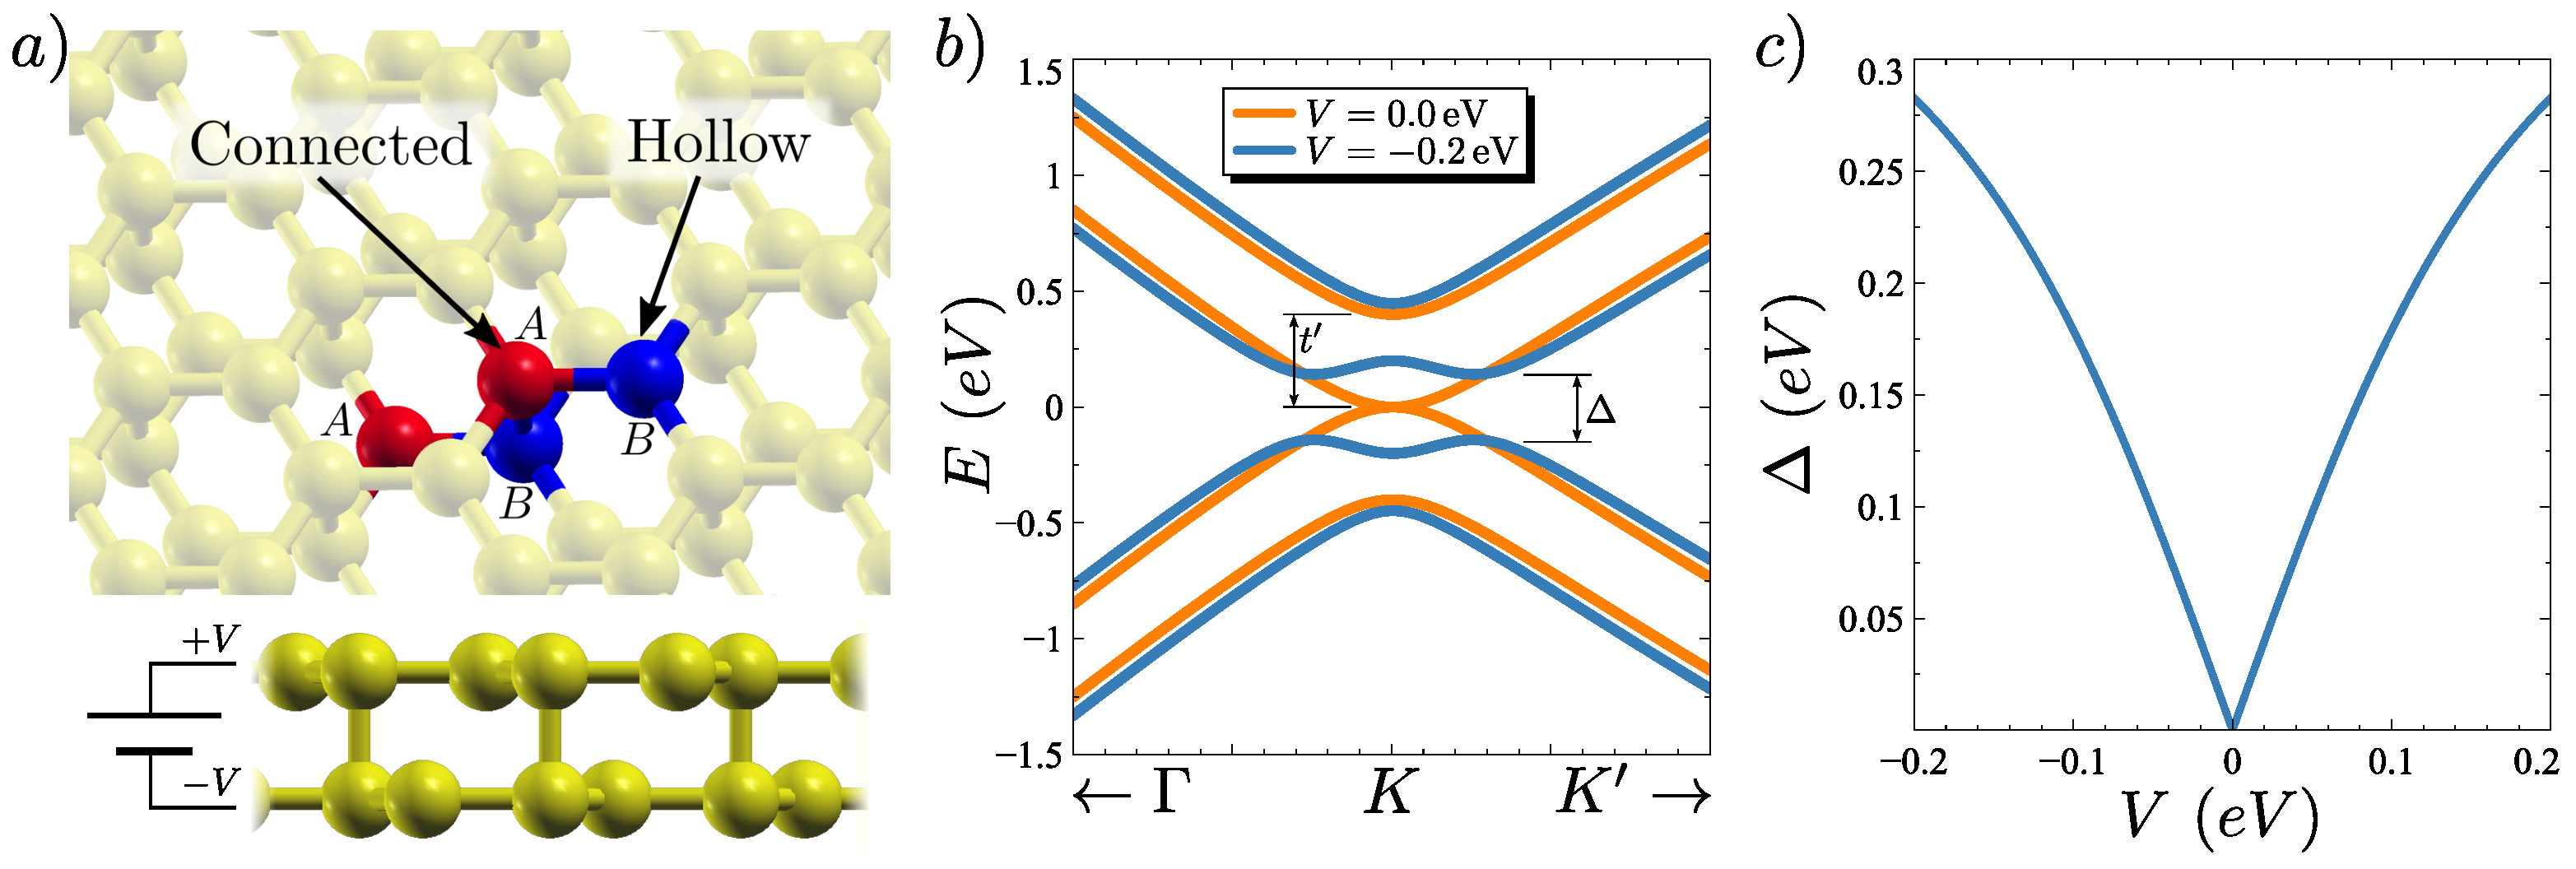
\includegraphics[width=0.9\textwidth]{artlat/fig/bands_bilayer.pdf}
\vspace{-5pt}
\caption{$a)$ Sketch of the minimal unit cell for graphene bilayer and disposition of the external electric field. Notice the two possibilities for placing the vacancies, we will focus on the hollow sites. $b)$ band structure of graphene bilayer with (blue) and without (orange) electric field. $c)$ Dependence of the gap open by the electric field. Notice that the gap is no longer at $K$, as shown in panel $b)$.}
\label{bilayer2d}
\end{figure}
% \FloatBarrier
%~~~~~~~~~~~~~~~~~~~~~~~~~~~~~~~~~~~~~~~~~~~~~~~~~~~~~~~~~~~%
Rather than having a linear band structure, bilayer graphene presents parabolic bands around the $K$ point. It has zero gap, and the next bands are split by the interlayer hopping $t'$. When an external electric field is switched on, a gap is open at the $K$ point as shown in Fig.~\ref{bilayer2d} $b)$ and $c)$. The band gap behaves linearly for small electric fields while it tends to saturation when the gap is comparable to the interlayer splitting governed by $t'$.

This calculation is not exactly accurate with the experimental results\cite{Zhang2009} since it does not consider any self-consistent or screening effect at all, nevertheless it contains the necessary ingredients to describe the relevant physics of the problem, so for the sake of simplicity we will remain at this level of description.



\subsection{Vacancies in Graphene bilayer}
When a single vacancy is placed in graphene bilayer (or graphene, for that matter), the translational invariance is broken. For this reason, we consider a finite hexagonal island with armchair edges. In order to neglect the edge effects we will use nano-islands as big as $\SI{50.6}{\nm}$ in diameter (over 130K atoms). %131772 atoms)
As it is expected, in such a system the confinement gap decreases linearly with the area of the island (quadratically with the side), as shown in Fig.~\ref{confinement} $a)$. This model will break down when the scale of the electric field becomes comparable to the confinement gap. We shall, then, stay clear of the small electric field regime in order to avoid finite size effects. Depending on the calculation different sizes for the island can be chosen with no major consequences.
%~~~~~~~~~~~~~~~~~~~~~~~~~~ FIGURE ~~~~~~~~~~~~~~~~~~~~~~~~~%
\begin{figure}[!ht!]
\centering
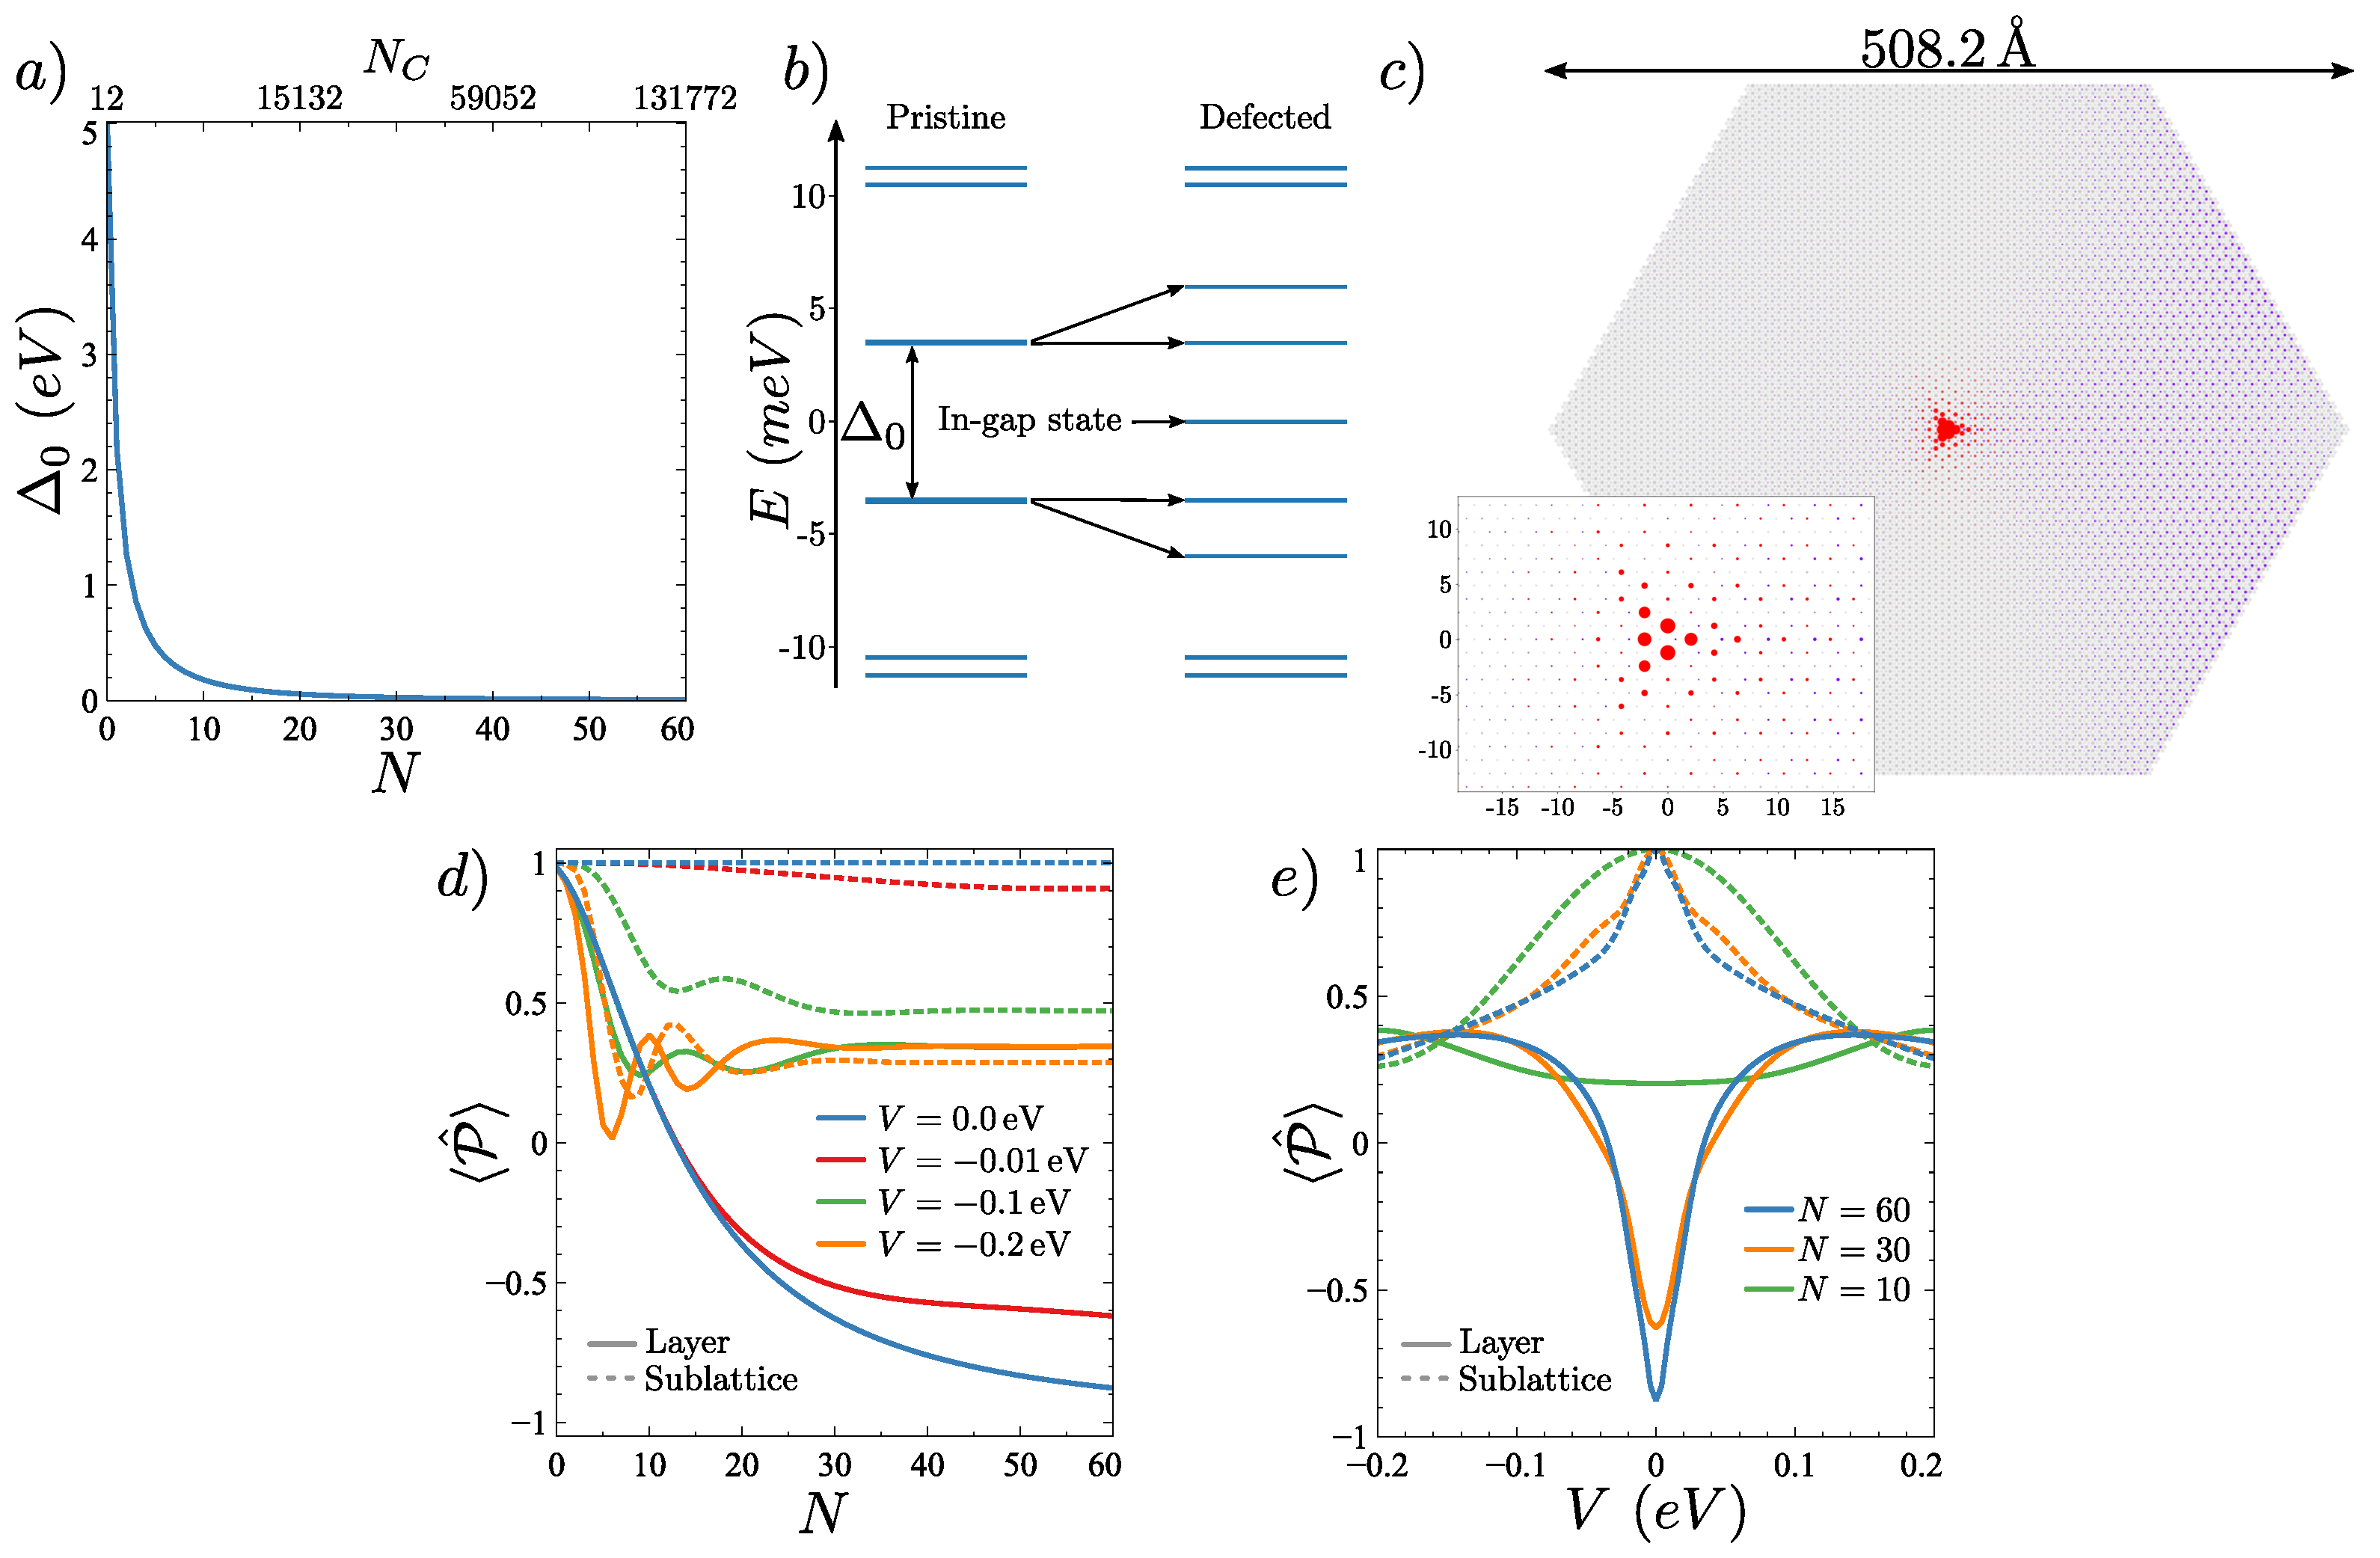
\includegraphics[width=\textwidth]{artlat/fig/confinement.pdf}
\vspace{-20pt}
\caption{$a)$ Confinement gap as a function of the size of the island (lower axis) and the number of carbon atoms $N_C$ in the island (upper axis). $b)$ Comparison of a pristine and a defected island, with a vacancy in the central hollow position. An in-gap state appears at zero energy. $c)$ Spatial distribution of the in-gap state. It appears distributed in both the top (red dots) and bottom layer (blue dots). Notice that the state is strongly localized around the vacancy in the top layer (red) while it is spread throughout the bottom layer (blue). The spatial distribution of the bottom layer is affected by the finite size of the sample and its exact shape is but a minor detail. The inset shows a $15\times\SI{10}{\angstrom}$ zoom of the in-gap state around the vacancy. $d)$ Dependence of the layer and sublattice polarizations with the size of the island. $e)$ Evolution of the layer and sublattice polarizations with the electric field for islands of different size.}
\label{confinement}
\end{figure}
% \FloatBarrier
%~~~~~~~~~~~~~~~~~~~~~~~~~~~~~~~~~~~~~~~~~~~~~~~~~~~~~~~~~~~%

We can calculate the spectrum of the system with and without a vacancy in order to compare both of them. Of course the full diagonalization of a $131772\times131772$ Hamiltonian is, at the very least, challenging for any standard computer, so we will use Lanczos diagonalization\cite{Lanczos1950, Ojalvo1970, Arnoldi1951} to obtain only the 9 eigenvalues closest to the Fermi energy.

As shown in Fig.~\ref{confinement} $b)$ the main difference when the vacancy is introduced is that a state appears in the middle of the (confinement) gap. As a matter of fact there will appear as many in-gap states as vacancies are introduced.

When we analyze the in-gap state we see that it is $100\%$ sublattice polarized, as predicted by the Lieb's theorem\cite{Lieb1989}. Regarding the layer distribution, it is distributed in both layers but not equitably. Interestingly, the in-gap state has more spectral weight in \textbf{the layer that does not host the vacancy} and the bigger the island, the stronger this polarization is as shown in Fig.~\ref{confinement} $d)$.
We can check the spatial distribution of this state (see Fig.~\ref{confinement} $c)$) to see that it is actually quite localized in the top layer (red dots), but completely spread over the bottom layer (blue dots). The particular shape of the distribution of the bottom layer is strongly affected by the edges so it is not to be considered as a reliable result, nevertheless its spreading (calculated via IPR later) is consistent through different shapes and island sizes, and in accordance to the literature\cite{Castro2010}.

%TODO discuss <S> with size

\subsection{Note on the geometry}
All the vacancies considered will always be chosen on a hollow position (see fig~\ref{geo_sketch} $c)$) even if it not specified in the text. The behavior of vacancies in connected sites is studied somewhere else\cite{Castro2010}.

When only one vacancy is considered, it will be placed at the (hollow) atomic position closest to the center of the island in order to maximize the distance to the edges.

When two vacancies are considered, they will be placed as separated as possible from the edges, as shown in Fig.~\ref{geo_sketch} $b)$. This configuration (rather than placing one in the center, for instance) allows the study of a wider range of the angle, $\alpha$ and distance $d$.
When more than two vacancies are considered, they will be placed in the vertices of a regular polygon centered in the island.

% XXX For later, when talking about the angle
% Note that as long as the border effects are negligible, and due to the $C_3$ symmetry of the in-gap states in graphene, we only need to explore the range of angles between vacancies of $\alpha\in\left[0,60\right]$.

%~~~~~~~~~~~~~~~~~~~~~~~~~~ FIGURE ~~~~~~~~~~~~~~~~~~~~~~~~~%
\begin{figure}[h!]
\centering
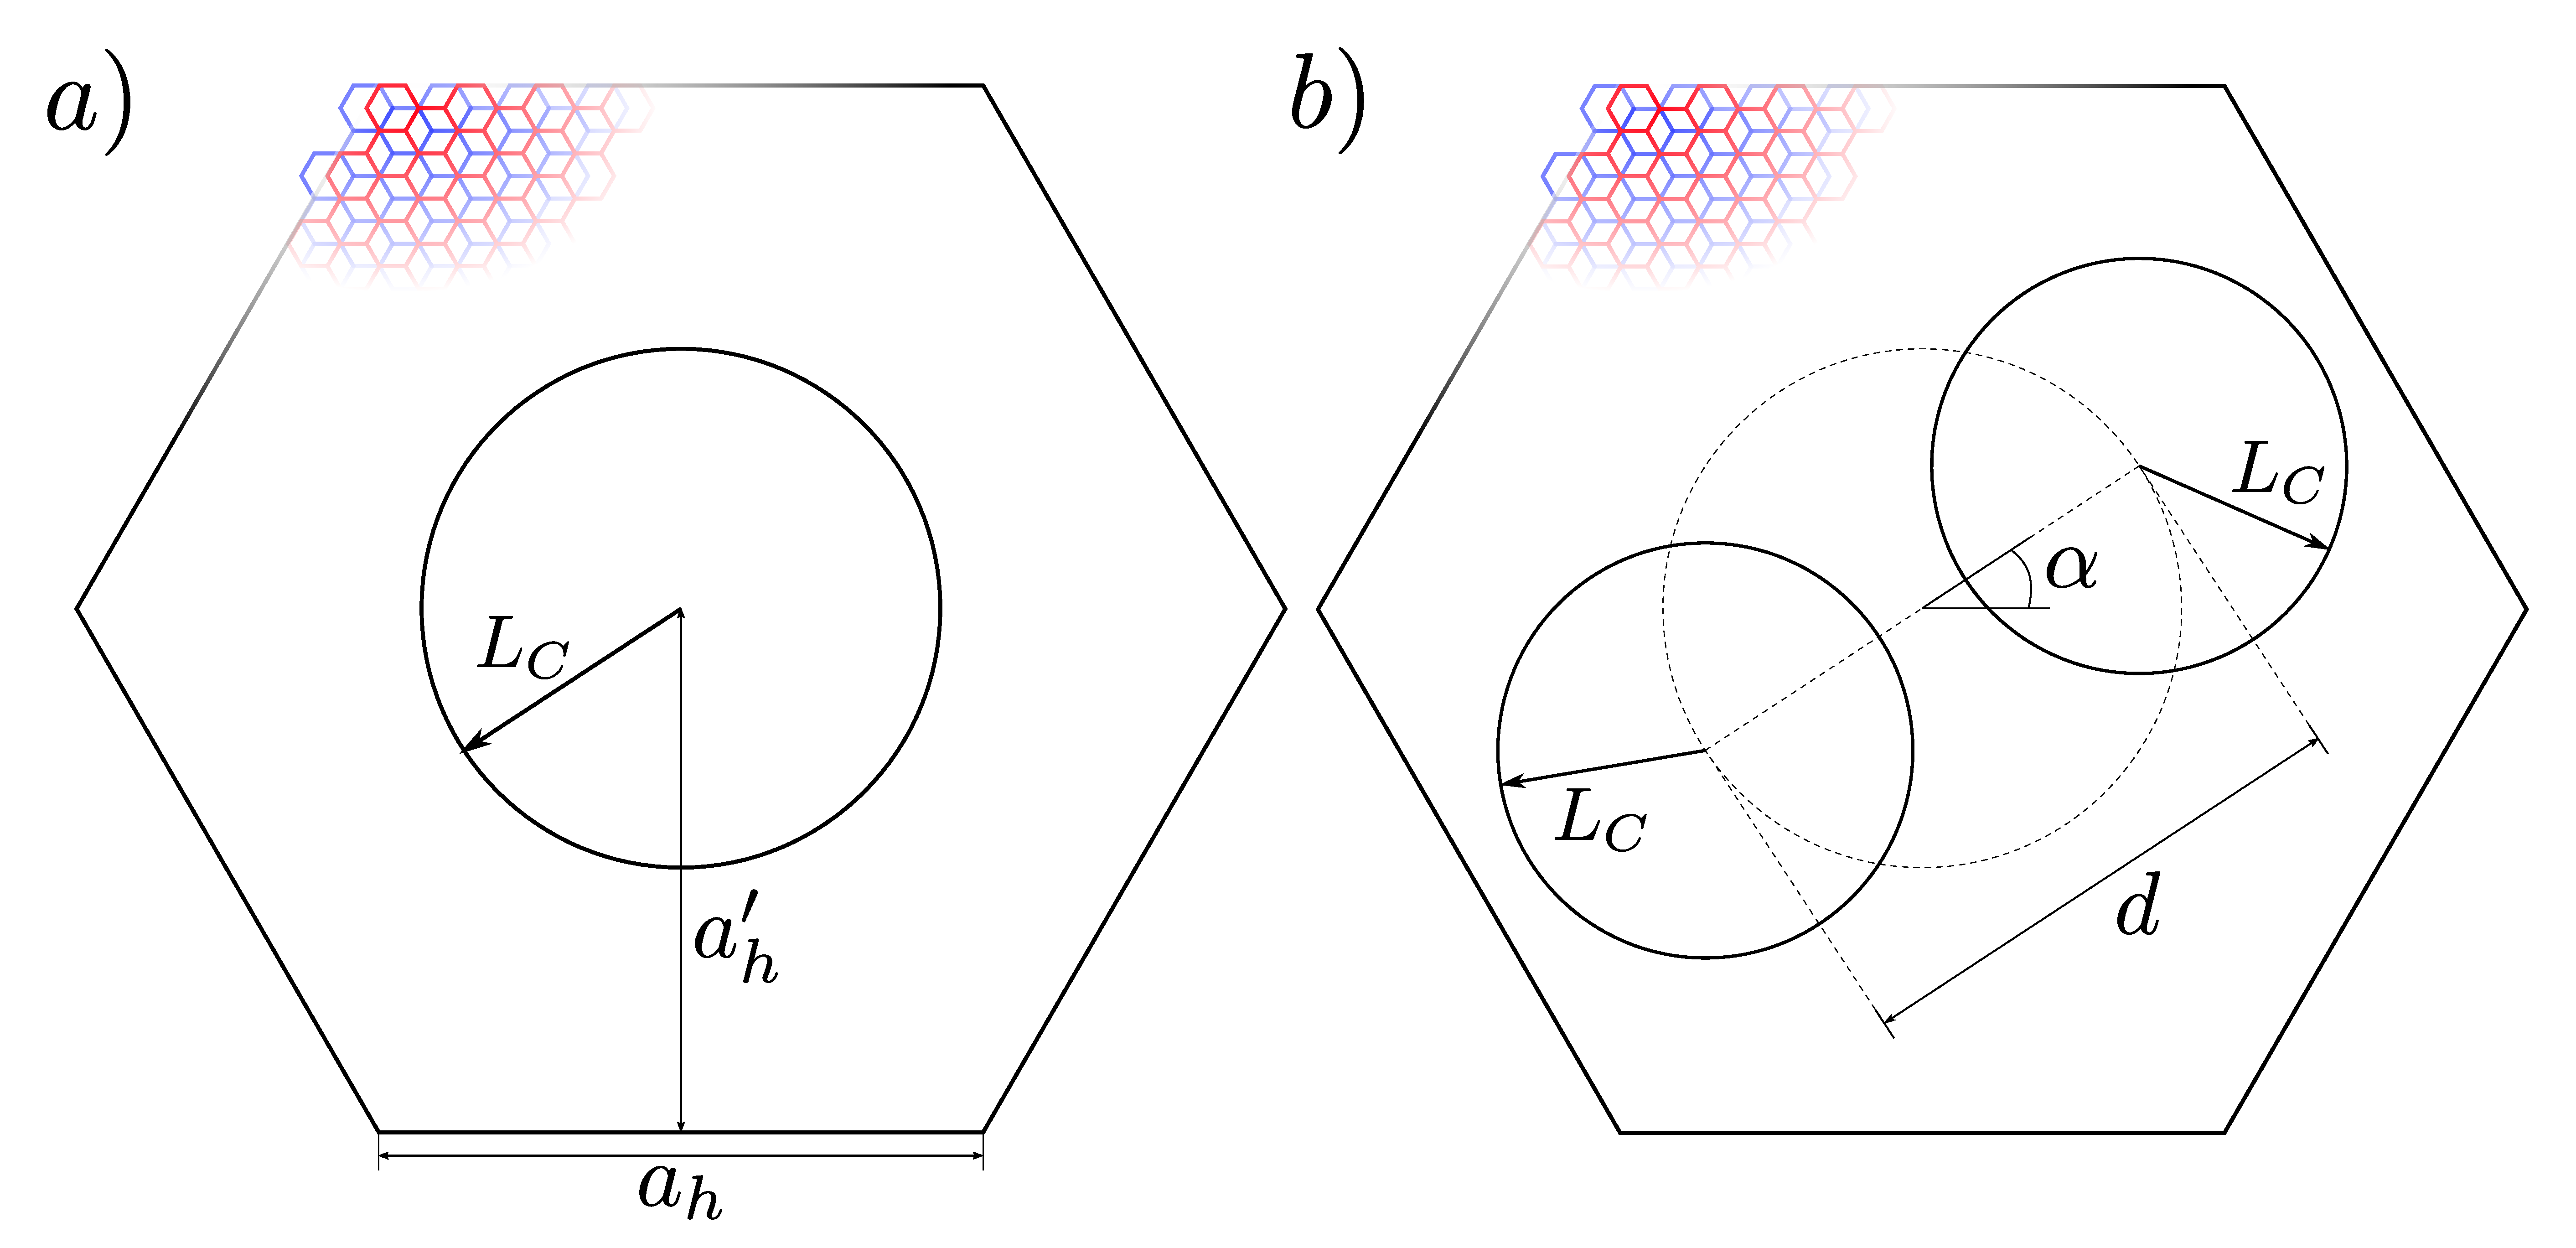
\includegraphics[width=0.7\textwidth]{artlat/fig/vacs_sketch.pdf}
\vspace{-10pt}
\caption{$a)$ and $b)$ show sketches of the position of the vacancies and relevant geometric information. In the upper left corner the real atomic structure is shown using blue for the lower layer and red for the upper one. The length $L_C$ is the typical size of the in-gap state.} % $c$ atomic structure showing the ``connected'' and ``hollow'' sites in the upper layer as well as the $A/B$ sublattices (in red/blue).}
\label{geo_sketch}
\end{figure}
\FloatBarrier
%~~~~~~~~~~~~~~~~~~~~~~~~~~~~~~~~~~~~~~~~~~~~~~~~~~~~~~~~~~~%




\section{0-D. Electric control of a single vacancy} %~~~~~~~~~~~~~~~~~~~~~~~~~~%
When an electric field is applied to bilayer graphene with a vacancy, the in-gap state will no longer be at zero energy. Instead, its position will shift with the electric field. As stated before, in a finite island we cannot define Bloch vectors, so we do not have bands. Nevertheless we can plot the spectrum of the island for different electric fields next to each other, this way we can have a band-looking plot showing the smooth evolution of the energy levels with the external potential.
%~~~~~~~~~~~~~~~~~~~~~~~~~~ FIGURE ~~~~~~~~~~~~~~~~~~~~~~~~~%
\begin{figure}[!ht!]
\centering
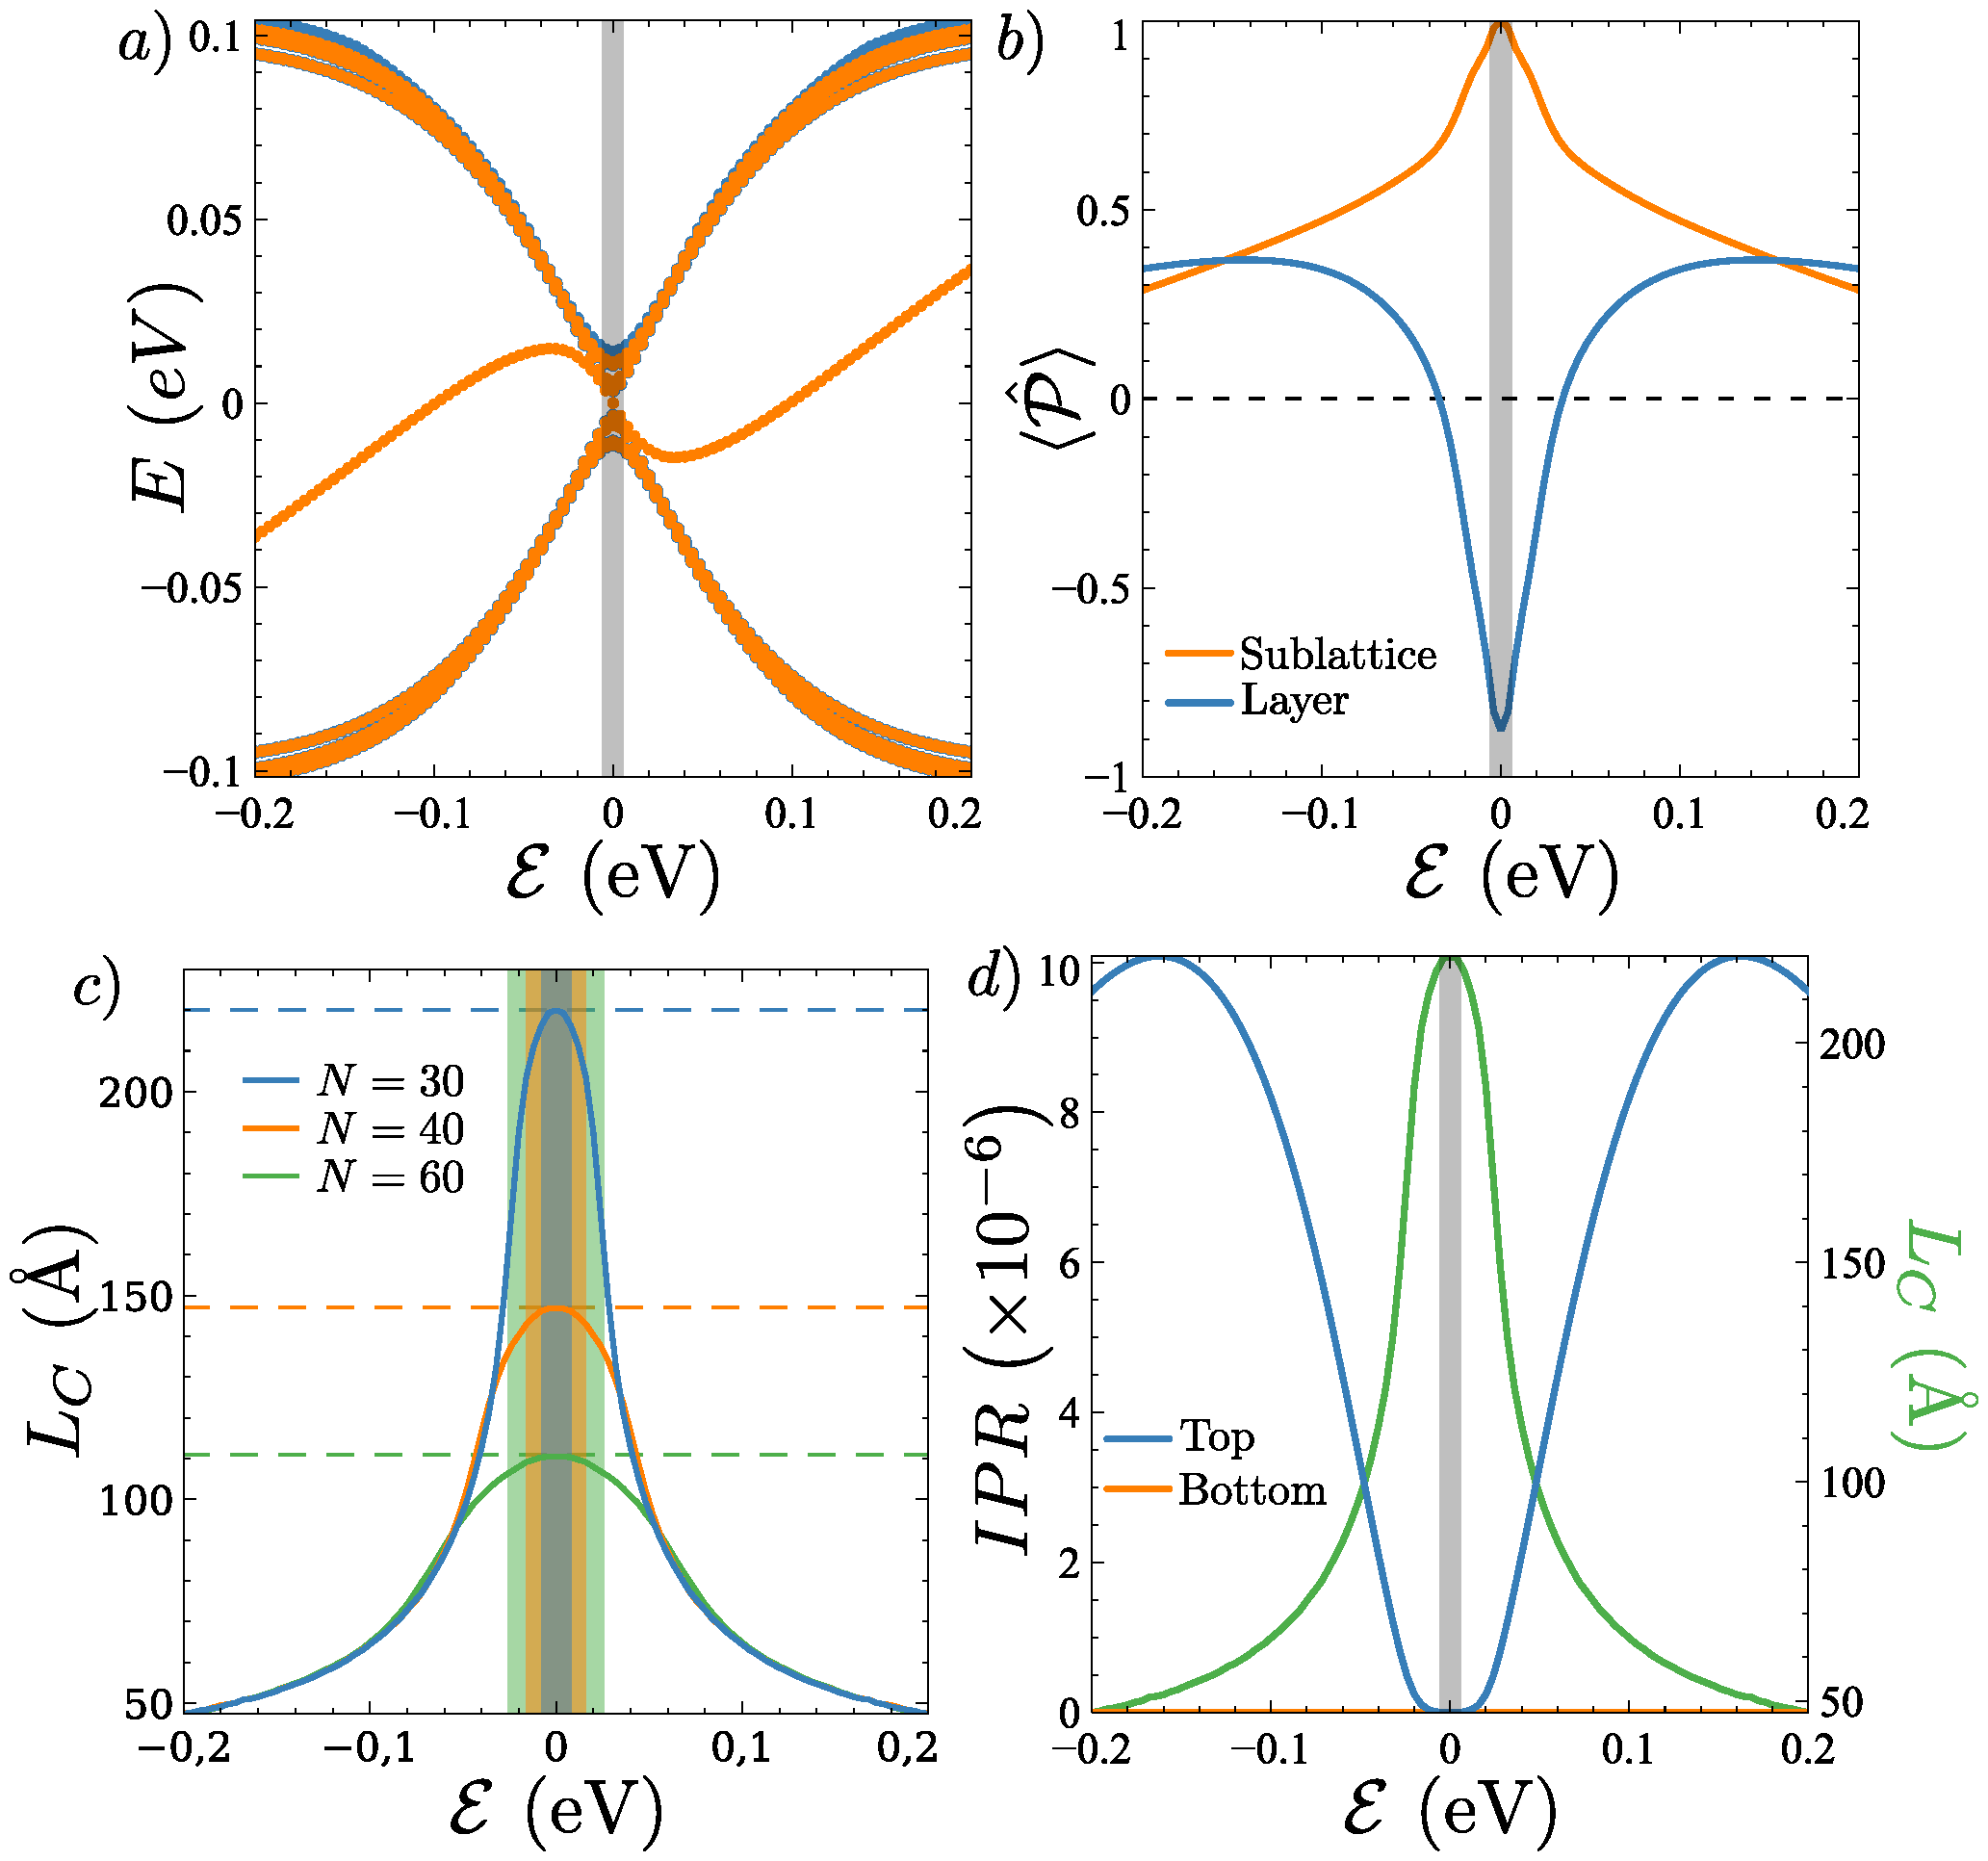
\includegraphics{artlat/fig/spectrum.pdf}
\vspace{-20pt}
\caption{$a)$ Evolution of the spectrum of an armchair island with the electric field. $b)$ Sublattice and Layer polarization as a function of the electric field. $c)$ Evolution of the IPR for the top (blue) and bottom layer (orange) and confinement length (green) with the electric field. Notice that the IPR for the bottom layer is very close to zero ($IPR_b\sim10^{-11}$) while the for the top layer it changes five orders of magnitude with the electric field, showing how much the in-gap state can be confined. Analogously the confinement length shows (right axis) that the state is spread all over the island for $V=\SI{0}{\eV}$ but it can be confined to $\sim\SI{50}{\angstrom}$. The vertical gray strip in all panels shows the region where $|V|\leqslant\Delta_0$, where the edge effects can play a role.}
\label{spectrum}
\end{figure}
% \FloatBarrier
%~~~~~~~~~~~~~~~~~~~~~~~~~~~~~~~~~~~~~~~~~~~~~~~~~~~~~~~~~~~%
In Fig.~\ref{spectrum} we see the evolution of different properties with the electric field. Panel $a)$ shows the deformation of the spectrum of the island with the electric field. The in-gap state appears consistently in the middle of the gap but its position does not change monotonously. There is an interplay between the charge polarization and the external electric field.
As the electric fields becomes stronger, we can see that the in-gap state looses its initial polarization, Fig.~\ref{spectrum} $b)$, reaching a stable distribution of between both layers and sublattices. Another effect introduced by the electric field is the localization of the state. Fig.~\ref{spectrum} $c)$ shows the strong reduction of the confinement length, $L_c$, defined as:
\begin{equation}
  0.98 = \int_{r_0}^{L_C} \Psi_0(r) dr   %XXX arreglar!!!
\end{equation}
This non-standard definition gives an intuitive idea of how far from the vacancy (placed at $r_0$) is most of the state (over $90\%$ of it).
It is interesting to notice that the inverse participation ratio, $IPR$, defined as:
\begin{equation}
  \ket{\Psi_0} = \sum_\beta c_\alpha\ket{\phi_\alpha}\quad\quad;\quad\quad
  \text{IPR} = \sum_\alpha |c_\alpha|^4
\end{equation}
behaves quite differently for the top and bottom layer. Let us keep in mind that the smaller the $IPR$, the more spread the state is, in the limit case in which a given state is spread over all the $N$ available atoms, the $IPR$ would be $IPR=1/N$, while for a state localized in a single atom, it would be $IPR=1$.
For the bottom layer, the $IPR$ is very small and it barely changes with the electric field. This shows an extended state no matter the applied electric field. That is not the case for the top layer. In the top layer the $IPR\sim0$ for very small electric fields, but it increases rapidly with the electric field, showing that the state gets quickly localized. This is also confirmed by looking at the confinement length (green line in Fig.~\ref{spectrum} $c)$) which begins at a huge value, comparable to the size of the island, and decreases to a few nanometers.


A first order perturbative calculation of the energy at which the in-gap state should appear yields
\begin{equation}
  E_0 (V) = V \bra{\Psi_0}\hat{L}\ket{\Psi_0}
\end{equation}
In order to understand the implications of this, let us consider a vacancy in the upper layer ($\lambda_l=+1$). At $V=\SI{0.0}{eV}$, the in-gap state, $\Psi_0$, is quite layer-polarized: $\bra{\Psi_0}\hat{L}\ket{\Psi_0}\sim-0.8$. When the electric field is switched on, the in-gap state shifts with a negative slope. Nevertheless the electric field opposes the starting polarization and eventually they cancel out, which results in a change of sign in the slope. % XXX pufff.... rewritte

This behavior suggests a crossover between two interactions: the electric field and the kinetic terms. Let us study the effects of the interlayer coupling in this system.


\subsection{Role of the interlayer coupling}
Naively, one may expect the in-gap state to shift linearly with the electric field as, for instance, the conduction and valence states do. Nevertheless, the calculations show otherwise.
For small electric fields (we will discuss this scale later on) the in-gap state moves in opposition to the electric field, as discussed in Fig.~\ref{spectrum} $a)$.
%~~~~~~~~~~~~~~~~~~~~~~~~~~ FIGURE ~~~~~~~~~~~~~~~~~~~~~~~~~%
\begin{figure}[!ht!]
\centering
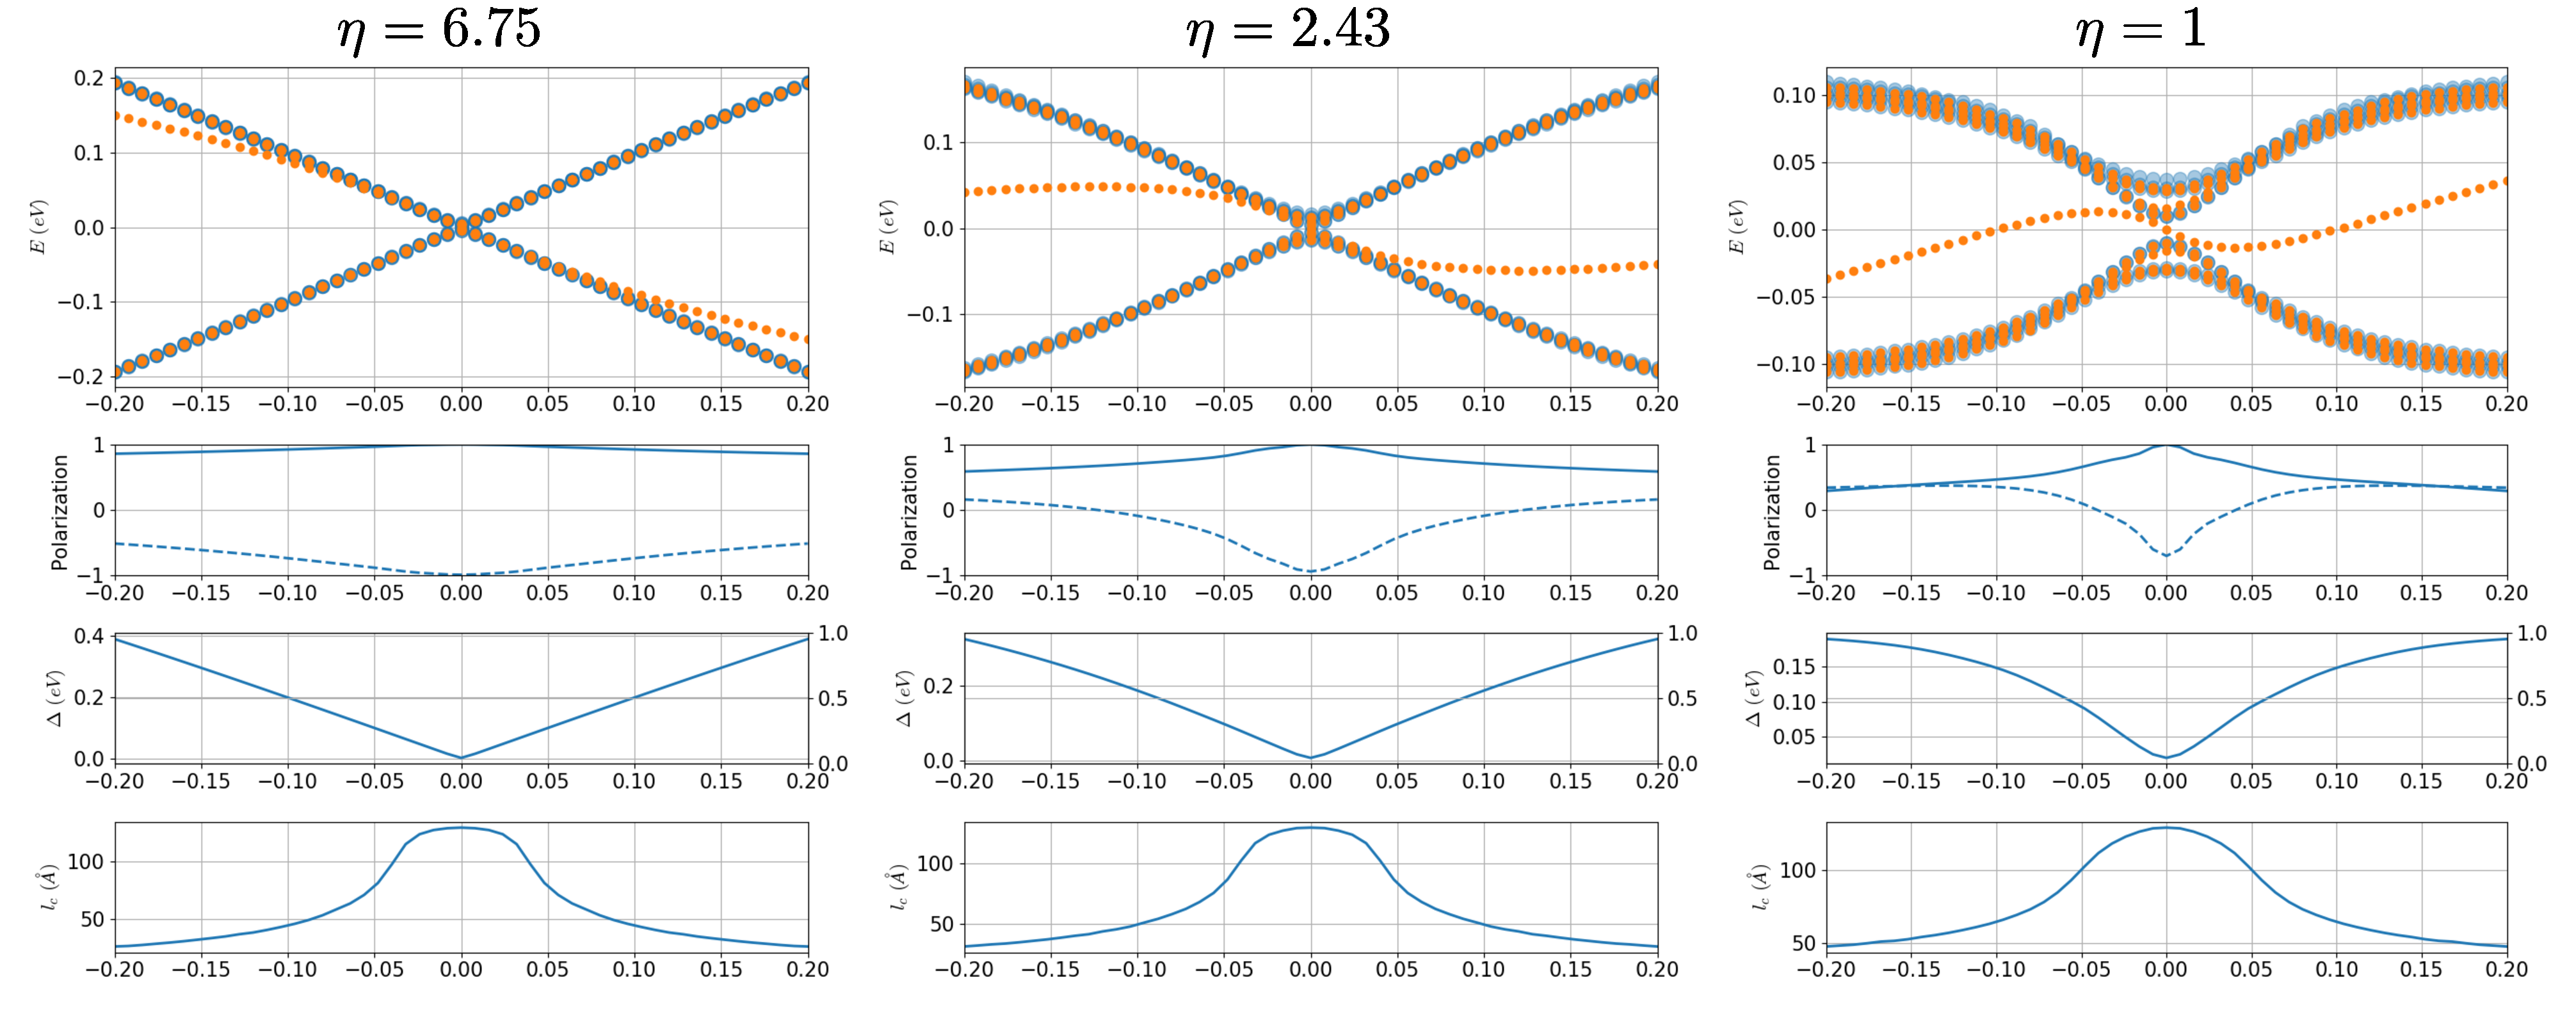
\includegraphics{artlat/fig/ingap_interlayer.pdf}
\vspace{-15pt}
\caption{Evolution of the spectrum with the interlayer coupling. The left panel shows the spectrum if we consider interlayer interactions as strong as the intralayer ones. The right panel shows the realistic value and the central panel shows an intermediate situation.}
\label{ingap_interlayer}
\end{figure}
% \FloatBarrier
%~~~~~~~~~~~~~~~~~~~~~~~~~~~~~~~~~~~~~~~~~~~~~~~~~~~~~~~~~~~%
For large electric fields the in-gap state does move linearly with the electric field, yet, the rate at what it does depends strongly on the interlayer coupling, as shown in Fig.~\ref{ingap_interlayer}.
We will consider the Hamiltonian of the system to be two graphene hamiltonians coupled by an interlayer interaction:
\begin{equation}
  H = H_{\text{L}_1} + \eta H_{\text{inter}} + H_{\text{L}_2}
\end{equation}
The intralayer $\pi$-hoppings are $t=\SI{-2.7}{\eV}$ while the interlayer hoppings (which are $\sigma$-hoppings, due to the symmetry of the orbitals) are roughly $t_{\text{inter}}=\SI{0.4}{\eV}$. $\eta$ is an artificial adimensional parameter that will allow us to tune the interlayer coupling to study the behavior of the system. In this fashion, $\eta=1$ corresponds to normal, realistic GBL, while $\eta=0$ describes two decoupled graphene layers and, in particular, $\eta=6.75$ corresponds to having an \emph{inter}layer coupling as strong as the \emph{intra}layer one.\\

In order to understand the role of the interlayer coupling in the in-gap state, it is useful to plot the dependence of the layer polarization with the parameter $\eta$. We consider this parameter to range from 0.5 (slightly decouple) to 6.75 (strongly coupled so inter and intralayer hopping is the same).
%~~~~~~~~~~~~~~~~~~~~~~~~~~ FIGURE ~~~~~~~~~~~~~~~~~~~~~~~~~%
\begin{figure}[!ht!]
\centering
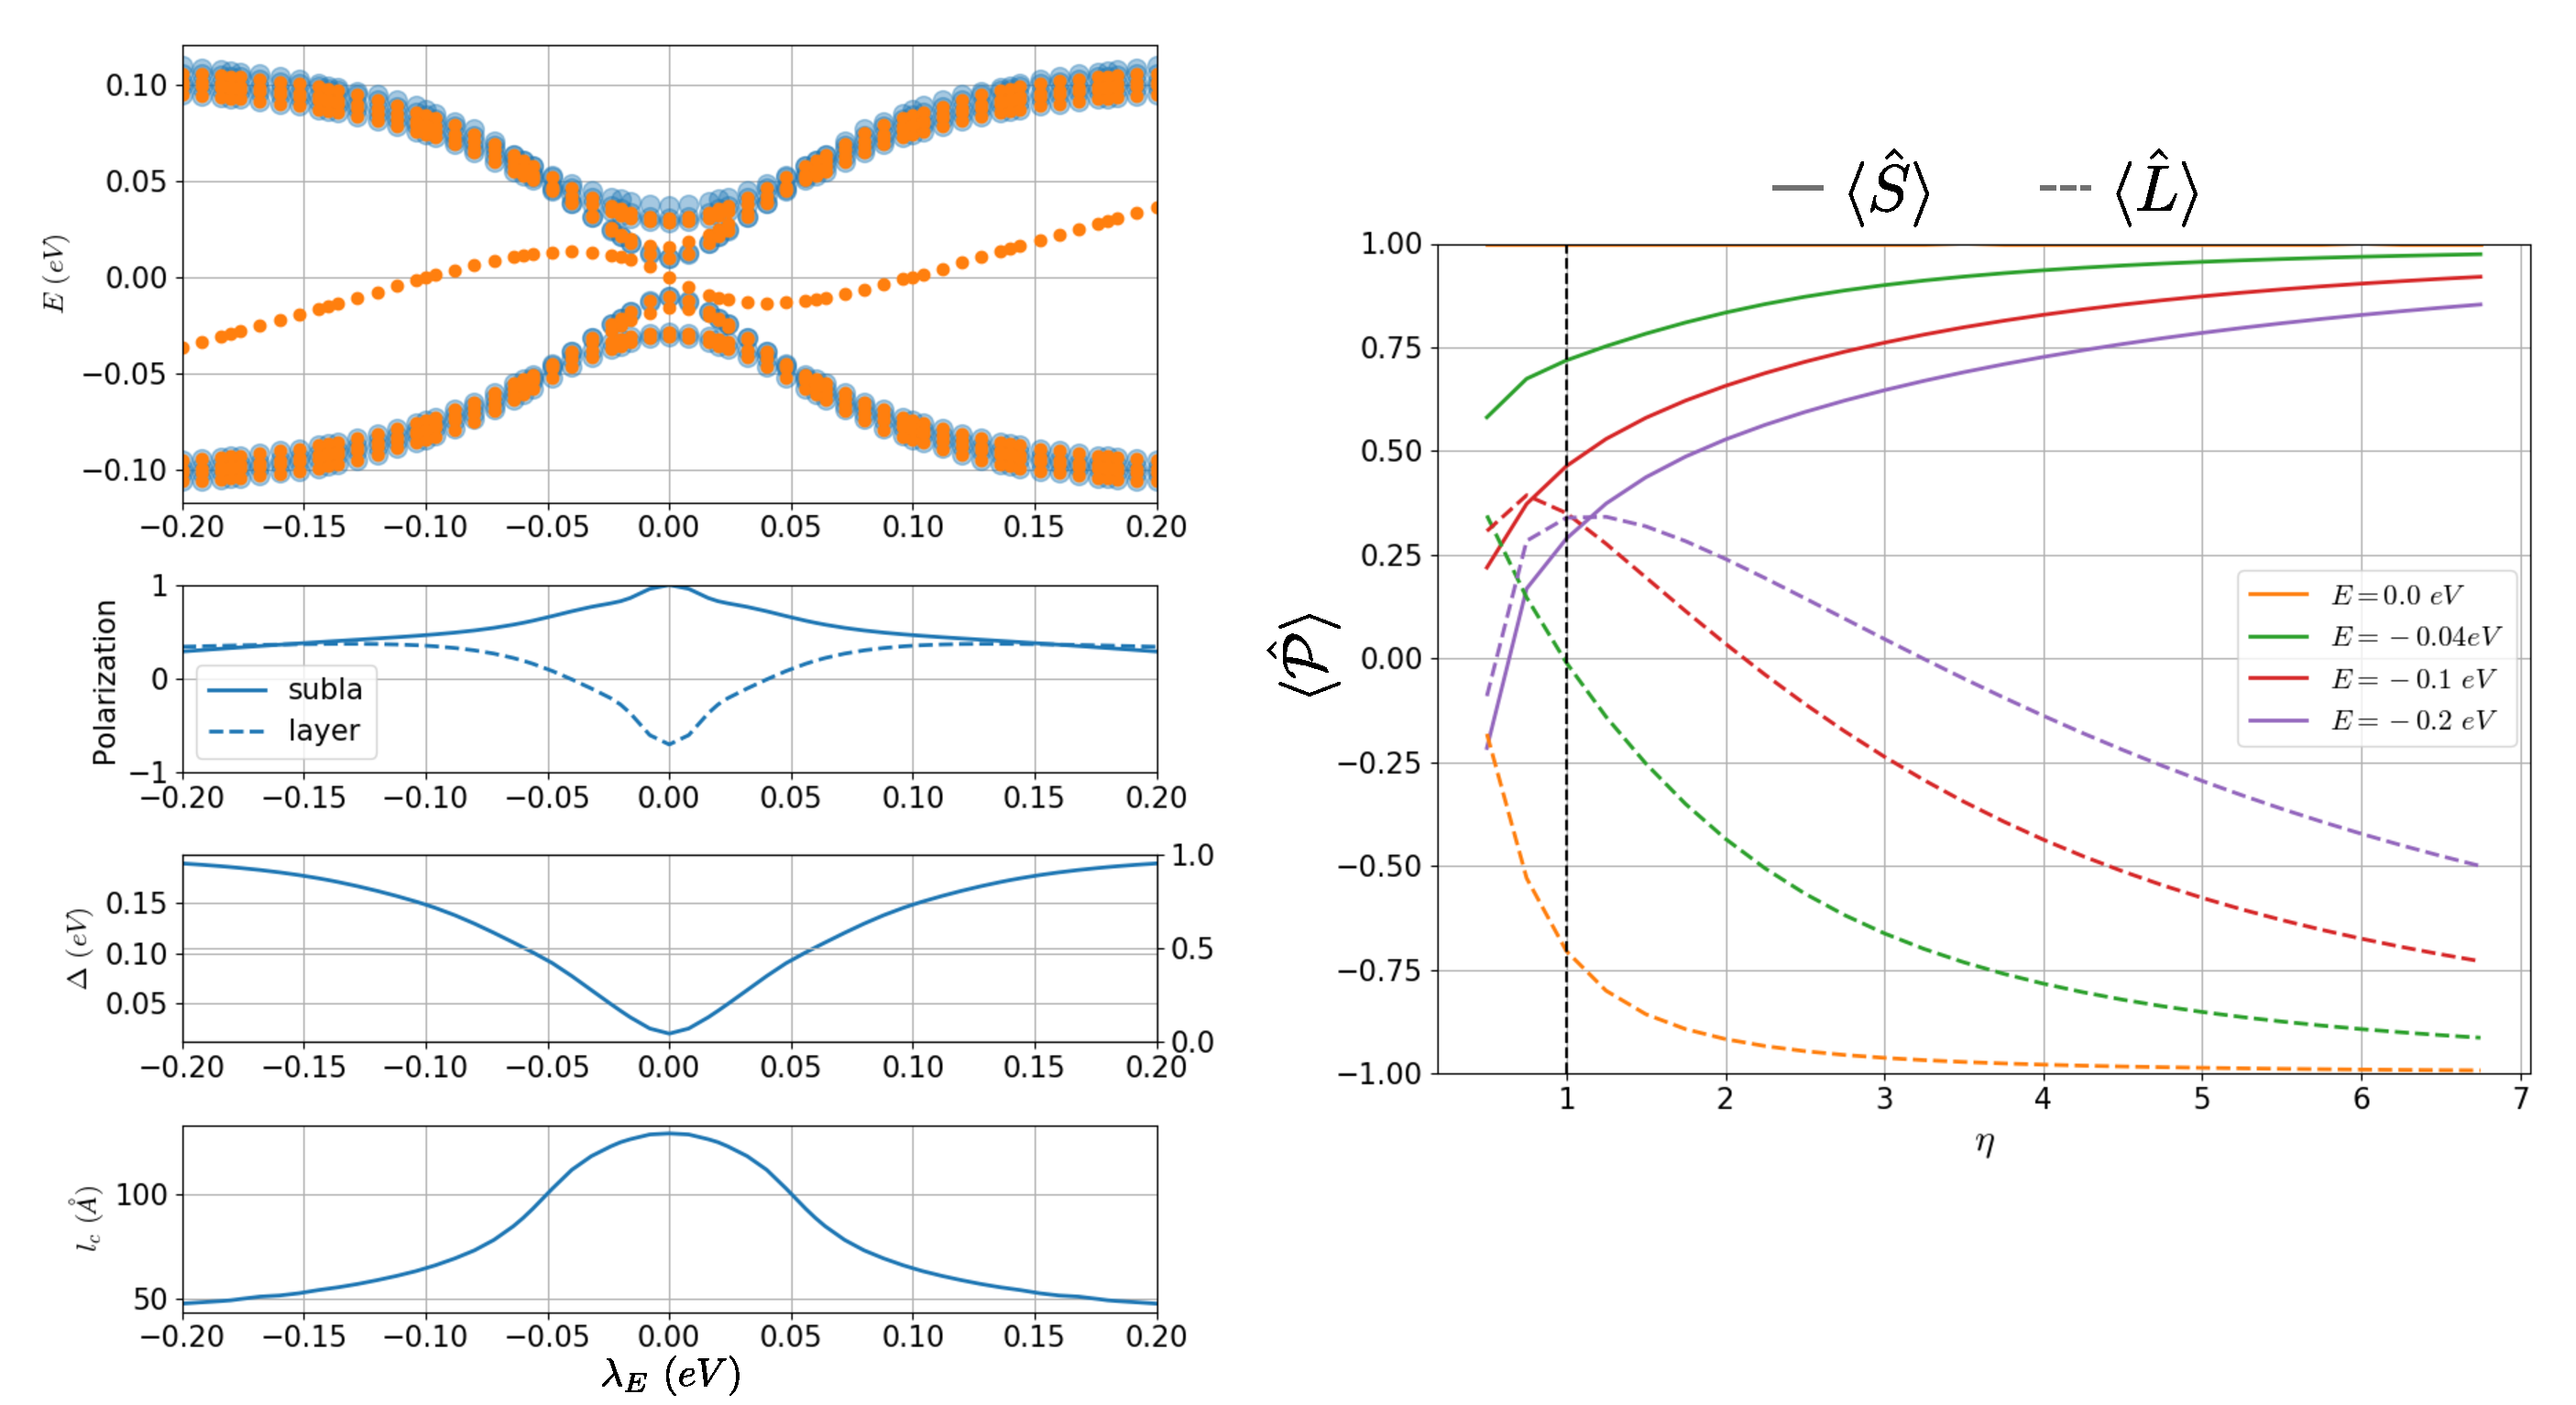
\includegraphics[width=\textwidth]{artlat/fig/polarization.pdf}
\vspace{-15pt}
\caption{$a)$ Evolution of different properties with the electric field. First panel shows the evolution of the spectrum, the second one shows the sublattice and layer polarizations, the third one plots the gap of the system and the forth one shows the confinement length. $b)$ Evolution of the layer (dashed lines) and sublattice polarization (solid lines) with the interlayer coupling. Notice that at zero electric field, $V=\SI{0.0}{\eV}$, the sublattice polarization remains constant at $\langle\hat{S}\rangle=1$, as expected from the Lieb's theorem.}
\label{pol}
\end{figure}
\FloatBarrier
%~~~~~~~~~~~~~~~~~~~~~~~~~~~~~~~~~~~~~~~~~~~~~~~~~~~~~~~~~~~%
We can see that the electric field overcomes the interlayer contribution when the system reaches charge neutrality $\langle\hat{L}\rangle=0$.

We can try to understand this step by step. When a H adatom is introduced (aka, a vacancy), one electron is localized in the vicinity of the defect. %The three closest atoms bear most of the spectral weight of this state, and the rest spreads all over the island but only in one sublattice.
For an adatom chemisorbed on top of a C atom belonging to the sublattice -1 in the top layer (namely 1), the sublattice and layer polarization are:
\begin{equation*}
  \langle\hat{S}\rangle = 1 \quad;\quad
  \langle\hat{L}\rangle = -0.7
\end{equation*}

This means that the in-gap state is completely sublattice polarized (as Lieb's theorem predicts) but it is only $\sim70\%$ layer polarized, meaning that the localized electron lives mostly \textbf{in the layer that does not contain the vacancy}.

If we artificially increase the value of the interlayer coupling we can that the layer polarization consistently drops to lower values, showing that the in-gap state prefers to spread in the layer that does not contain the vacancy. Analogously, the evolution of the sublattice polarization also shows that the in-gap state gets more and more sublattice-polarized.

This behavior might be understood keeping in mind the behavior of a single vacancy in graphene. It is known that for a vacancy in graphene, the in-gap state is mostly concentrated in the three closest atoms. In graphene bilayer it happens that these three closest atoms are connected to the other graphene layer, so the stronger the interlayer coupling, the easier will be for the in-gap state to spread to the other layer.

What I do not understand is that the 3 atoms closest to the vacancy (containing most of the state at $\eta=0$) are connected to atoms of the opposite sublattice in the other layer, yet, the sublattice polarization seems to keep its expected flavor even when the interlayer coupling is heavily increased.















% \newpage
% Since we are studying an island with a single vacancy, the energy levels are a discrete set of energies. In figure~\ref{1vac_spec} (c) the difference in the spectrum due to the introduction of a vacancy at $\lambda_E=0$ is shown. When a vacancy is introduced, an in-gap state appears at $E=0$ and some \emph{(quasi-)}degeneracies are broken.
%
% The effect of the electric field in the spectrum is shown in figure~\ref{1vac_spec} $a)$ and $b)$. Its main effect is to open a gap, linearly dependent with the electric field.
%
% The shift in the energy at which the in-gap state appears is linear for low electric field, but it remains in-gap for all the regime of electric fields studied. In fig~\ref{1vac_spec} $a$-$c)$ only the eight eigenvalues closest to $E=0$ are plotted. Nevertheless, since the spacing between levels is much smaller than the gap open by the electric field, they appear grouped in two sets of almost-degenerate energies, one at $E>0$ and the other at $E<0$.\\
%
% %~~~~~~~~~~~~~~~~~~~~~~~~~~ FIGURE ~~~~~~~~~~~~~~~~~~~~~~~~~%
% \begin{figure}[!ht!]
% \centering
% 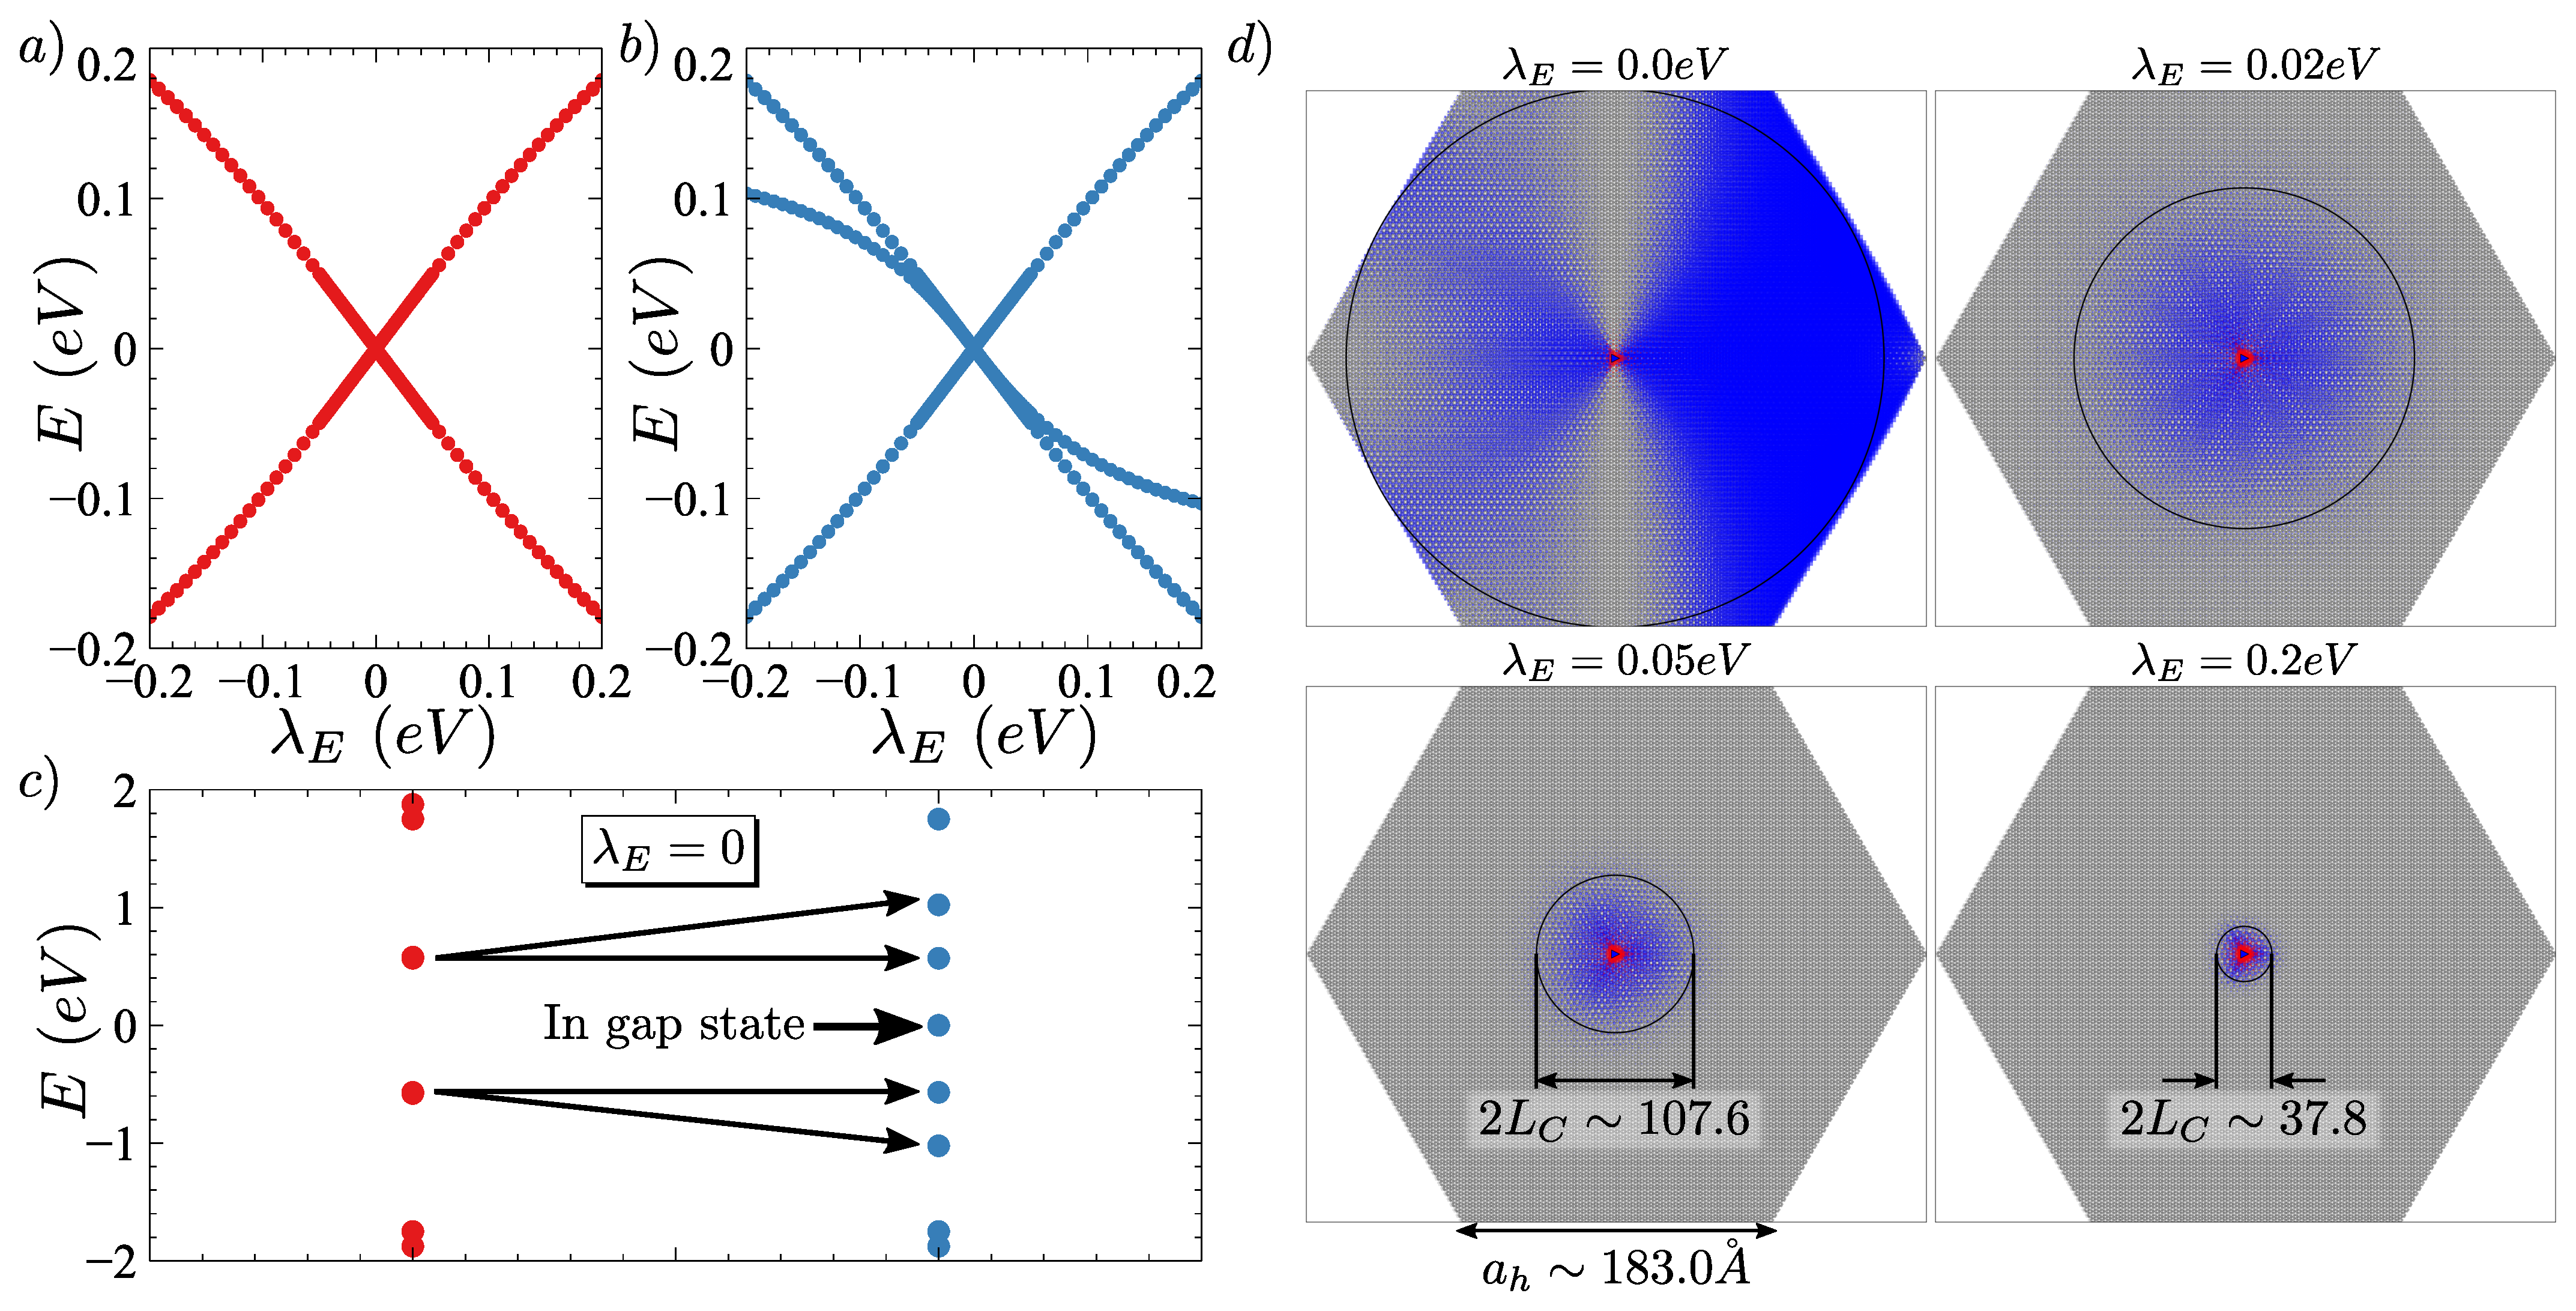
\includegraphics[width=\textwidth]{single_vac_spectrum.pdf}
% \vspace{-15pt}
% \caption{$a)$ and $b)$ show the pristine and defected spectrum respectively as a function of different applied electric fields. Notice the opening of a gap linear with the electric field (in both the pristine and defected cases) and the appearance of an extra state inside the gap. $c)$ Pristine (red) and defected (blue) spectrum for the case of no electric field $\lambda_E=0$. Panel $d)$ shows four snapshots of an island ($N_C=91812$ atoms) at different values of the electric field. The black circle in panel $d)$ shows the confinement length $L_C$ defined in the text.}
% \label{1vac_spec}
% \end{figure}
% \FloatBarrier
% %~~~~~~~~~~~~~~~~~~~~~~~~~~~~~~~~~~~~~~~~~~~~~~~~~~~~~~~~~~~%
%
% In Fig~\ref{1vac_spec} $d)$ we show four snapshots of the spatial distribution of the in-gap state. The actual lattice of the island is shown as black dots (probably indistinguishable because of the size of the image).
% On top of each atomic position the weight of the wave function ($|c_\beta|^2$ using the notation of eq.~\eqref{general}) is plotted in blue/red for the lower/upper layer.
% On top of all this, the site of the vacancy is marked with a blue triangle.
% As a visual guide the confinement length is plotted as a black circle with diameter $2L_C$.\\
%
% At $\lambda_E=0$ the system is bipartite, so according to the Lieb's theorem, after the removal of one site, a sublattice-polarized state should appear at $E=0$. This is exactly what happens as shown in Fig.~\ref{1vac_spec}.
%
% When we study the real-space distribution of the in-gap state we find that in the absence of electric field ($\lambda_E=0$) the state is spread all over the island, Fig.~\ref{1vac_spec} $d)$, no matter the size of the island (see Fig.~\ref{IPR_lc} $a)$ bellow). Notice that the effect of the border is not negligible in this regime and, in fact, is the responsible of the breaking of the expected $C_3$ symmetry of the state (at long distances, close to the vacancy the $C_3$ symmetry is almost preserved).
%
%
% Another important aspect is that the distribution of this wave function is such that in the upper layer (the one containing the vacancy) the wave function is quite confined around the vacancy (3-6 closest atoms) and it barely changes with the electric field, whereas in the lower layer the spreading of the wave function varies from the whole space available, to a few angstroms.
%
%
% To study quantitatively the properties of the in-gap state $\psi_0$ we define four quantities that will be useful later on.
% \begin{itemize}
%   \item \emph{Confinement length}, $L_C$, defined, hand-wavingly, as the distance at which more than $90\%$ of the state is located
%   \begin{equation}
%     0.9 = \int_{0}^{L_C} \psi_0(r) dr   %XXX arreglar!!!
%     \label{loclen}
%   \end{equation}
%   This confinement length can be used as a measurement of the spreading of the in-gap state $\psi_0$.
%   \begin{equation}
%     L'_C = \bra{\psi_0} |R-r_0|^2\ket{\psi_0}
%   \end{equation}
%   \item \emph{Inverse participation ratio} (IPR), $\eta$. Using the notation of equation~\eqref{general}, the IPR can be defined as:
%   \begin{equation}
%     \ket{\psi_0} = \sum_\beta c_\beta\ket{\phi_\beta}\quad\quad;\quad\quad
%     \text{IPR} = \eta = \sum_i |c_\beta|^4
%   \end{equation}
%   \item \emph{Sublattice} and \emph{Layer polarization}, defined as the expected value of the in-gap state.
%   \begin{equation}
%     SP = \bra{\psi_0}\widehat{\mathcal{S}}\ket{\psi_0}
%     \quad\quad;\quad\quad
%     SL = \bra{\psi_0}\widehat{\mathcal{L}}\ket{\psi_0}
%   \end{equation}
%   where the operators $\widehat{\mathcal{S}}$ and $\widehat{\mathcal{L}}$ measure the component of a given state in a given sublattice and layer respectively. Both $SP$ and $SL$ have to be, by definition, in the closed interval $\left[-1,1\right]$.
% \end{itemize}
%
% In figure~\ref{IPR_lc} we study the dependence of these four properties, for different sizes of the island, as a function of the electric field.
% %~~~~~~~~~~~~~~~~~~~~~~~~~~ FIGURE ~~~~~~~~~~~~~~~~~~~~~~~~~%
% \begin{figure}[!ht]
% \centering
% 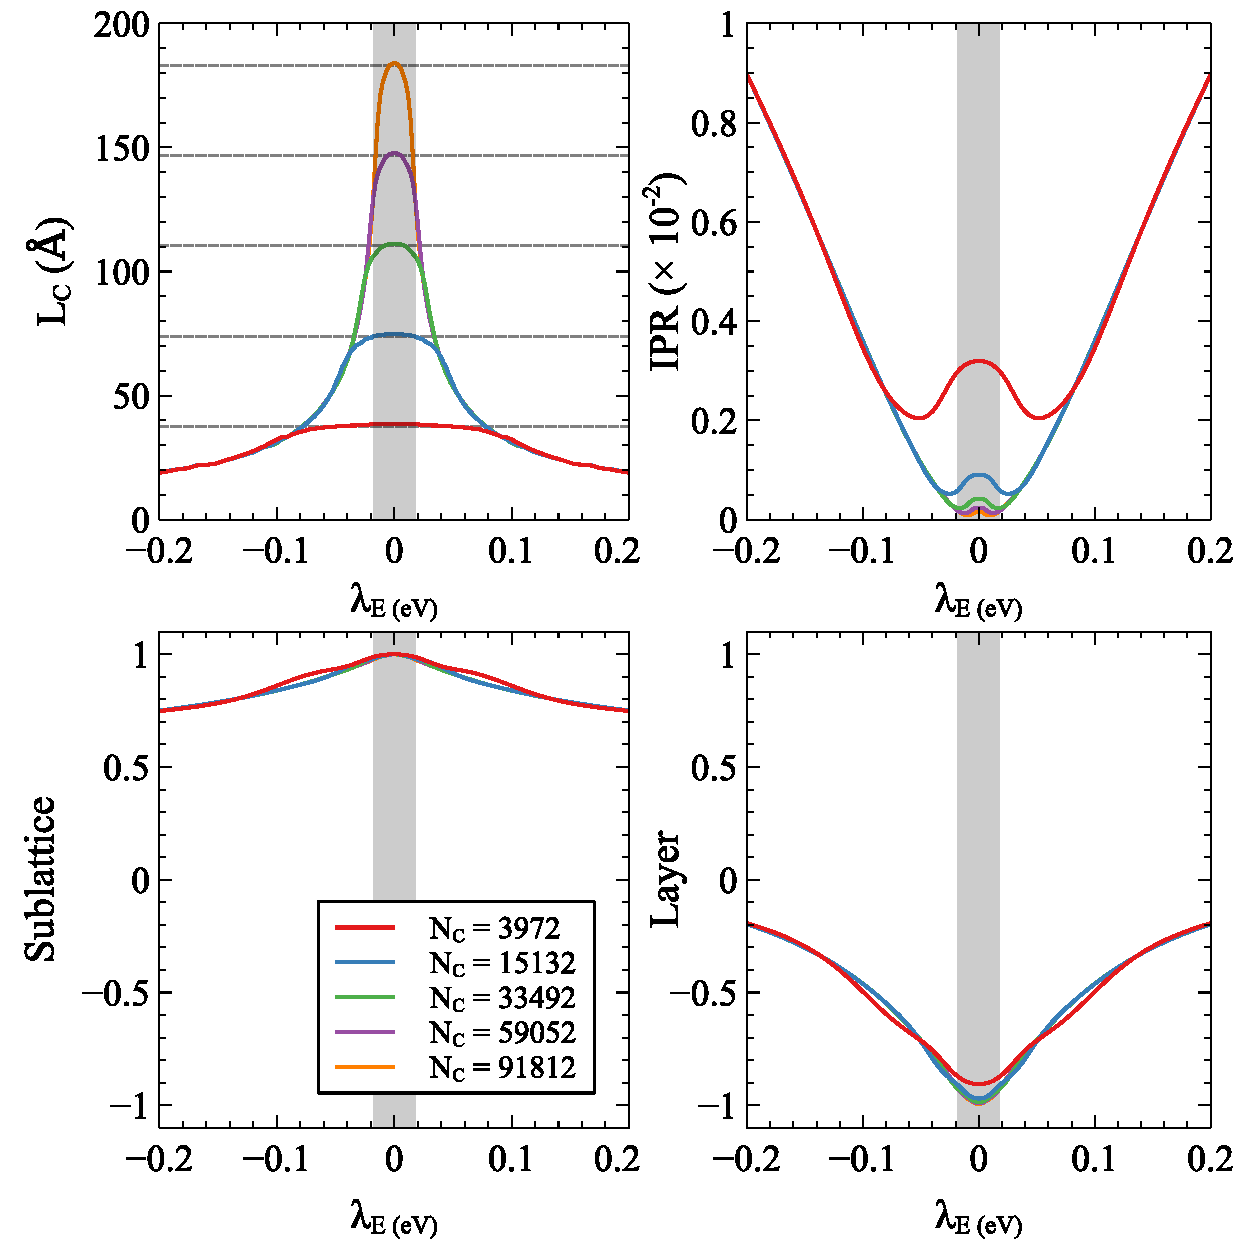
\includegraphics[width=0.6\textwidth]{single_vac_properties.pdf}
% \vspace{-5pt}
% \caption{$a)$ Dependence of the localization length $L_c$ with the electric field for different sizes of the island. The dashed lines corresponds to the size of the each corresponding island. $b)$ IPR, $\eta$, dependence with the electric field for different sizes of the island. $c)$ and $d)$ show the degree of sublattice and layer polarization for different sizes of the island as a function the electric field. The values $\pm1$ refer to $A/B$ sublattice or up/down layer respectively.}
% \label{IPR_lc}
% \end{figure}
% \FloatBarrier
% %~~~~~~~~~~~~~~~~~~~~~~~~~~~~~~~~~~~~~~~~~~~~~~~~~~~~~~~~~~~%
%
% It can be seen in Fig.~\ref{IPR_lc} $a)$ that as we approach the limit $\lambda_E\rightarrow0$ the confinement length collapses to the size of the island, shown as a dashed line for each size studied. This plateau is just the effect of having an in-gap state spread all over the island.
%
% The shadowed region in all the panels shows the range of $\lambda_E$ in which the border effects can be relevant for the biggest island studied ($N_C=91812$). It is estimated as the $\lambda_E$ at which the results differ from those of the previous island. Of course it is only a rough estimation and it should be considered only as a guide to the eye when reading the results.
%
% In panel $b)$ the IPR is shown. Except for small islands the evolution of the IPR, as that of the $L_C$, is the same regardless of the size of the island. The increasing of the IPR with the electric field is another sign of the increasing localization of the in-gap state around the vacancie.\\
%
% The sublattice and layer polarization are shown in panels~\ref{IPR_lc} $c)$ and $d)$. As it can be seen at $\lambda_E=0$ the state is completely sublattice-polarized, in accordance with the Lieb's theorem, and almost layer-polarized, this almost is more easly visible in the small red component present in Fig.~\ref{1vac_spec} $d)$.
%
% As the electric field increases the bipartite character of the system is lost, in agreement with the shift of the energy of the in-gap state (no longer at $E=0$). Since the system is no longer bipartite, the sublattice polarized character of the in-gap state is no longer assured, and as shown in panel $c)$ it, in fact, decreases.
%
% The decreasing of the layer polarization is easily understood by looking at Fig.~\ref{1vac_spec} $d)$. For small $\lambda_E$ the in-gap state is mostly spread over the lower layer, while for large $\lambda_E$ the in-gap state occupies roughly the same area in both layers resulting in a $\bra{\psi_0}\widehat{\mathcal{L}}\ket{\psi_0} \rightarrow 0$
%
%
%
%
% % When a single $p_z$ site is removed from graphene, an electron is confined in the surroundings of the vacancy with energy $E=0$. While it is true that such a state is mainly localized in the 3 closest neighbors, the rest of the state is diluted in all the other available sites. \red{[non-renormalizable?]}
% %
% % Interestingly, when a gap is open, the state becomes normalizable and a confinement length can be defined. In particular, the confinement length is controlled by the size of the gap.
% %
% % Graphene bilayer shows a tuneable band gap when an external electric field is applied\cite{}. This manipulation of the gap provides an excellent tool to control the confinement of any in-gap state.
% %
% % We will use an island of graphene bilayer with 91812 atoms. The removal of the hollow site closest to the center of the island results in an in-gap state as shown in Fig~\ref{single_vac}.
% %
% % %~~~~~~~~~~~~~~~~~~~~~~~~~~ FIGURE ~~~~~~~~~~~~~~~~~~~~~~~~~%
% % \begin{figure}[h!]
% % \centering
% %   \includegraphics[width=0.7\textwidth]{single_vacancy.pdf}
% % \vspace{-5pt}
% % \caption{Effect of an external electric field in the ingap state of a graphene bilayer with a single vacancy \red{include bands}}
% % \label{single_vac}
% % \end{figure}
% % \FloatBarrier
% % %~~~~~~~~~~~~~~~~~~~~~~~~~~~~~~~~~~~~~~~~~~~~~~~~~~~~~~~~~~~%

%~~~~~~~~~~~~~~~~~~~~~~~~~~ FIGURE ~~~~~~~~~~~~~~~~~~~~~~~~~%
\begin{figure}[h!]
\centering
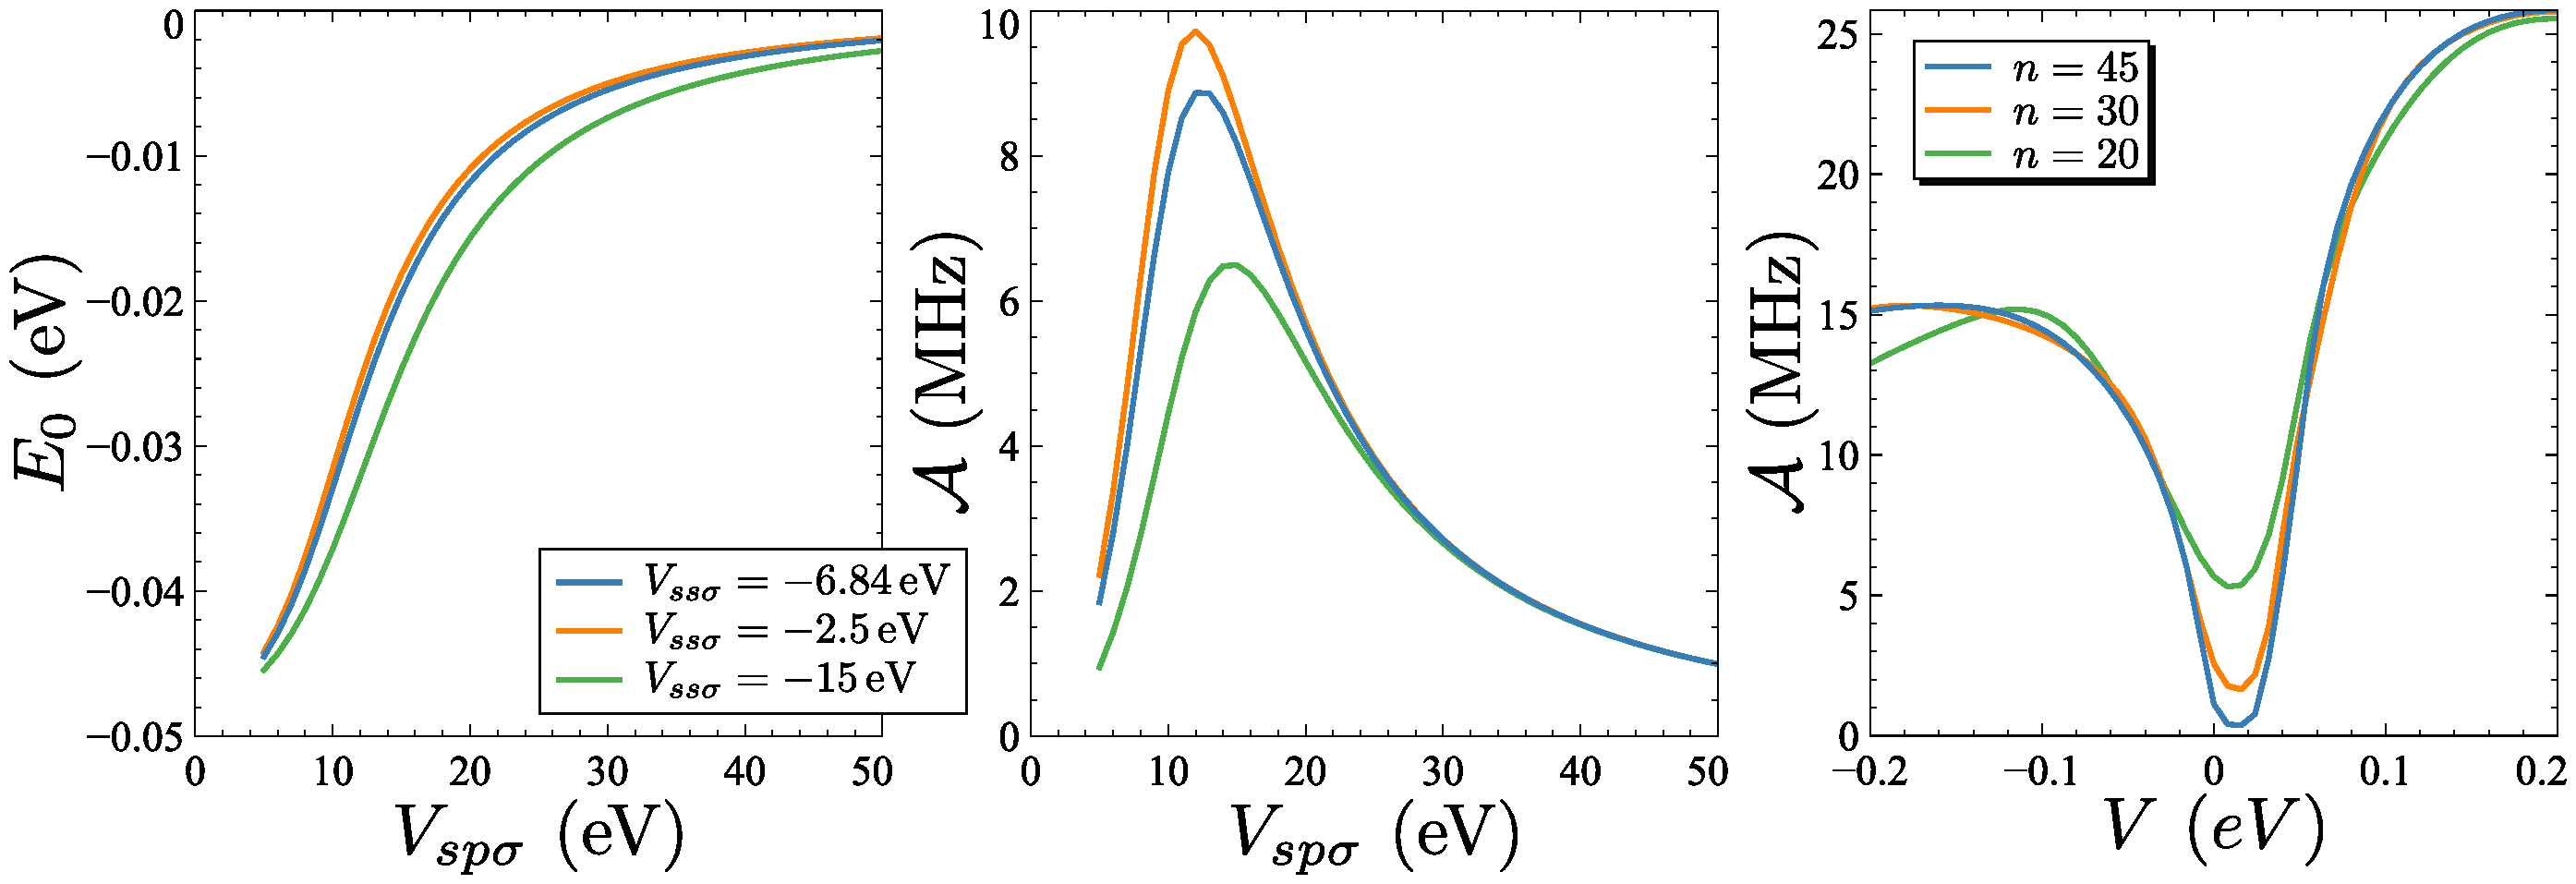
\includegraphics{artlat/fig/hyperfine.pdf}
\vspace{-20pt}
\caption{Change in the hyperfine coupling with the electric field.}
\label{latt_hyper}
\end{figure}
\FloatBarrier
%~~~~~~~~~~~~~~~~~~~~~~~~~~~~~~~~~~~~~~~~~~~~~~~~~~~~~~~~~~~%



\section{2-D. Designer fermion lattices} %~~~~~~~~~~~~~~~~~~~~~~~~~~~~~~~~~~~~~%
\subsection{The Geometry}
Since we require vacancies to be placed only in hollow positions, its possible placements form a triangular lattice \red{($C_6$ symmetry?)}. By carefully choosing the location of the vacancies, many different meta-lattices may appear.
%The artificial lattices that we can build by choosing the correct placing of the vacancies can form almost all the 2D Bravais lattices. \fref{art_lattices}
%%~~~~~~~~~~~~~~~~~~~~~~~~~~ FIGURE ~~~~~~~~~~~~~~~~~~~~~~~~~%
%\begin{figure}[h!]
%\centering
%\includegraphics{path/to/file.ext}
%\vspace{-5pt}
%\caption{Some examples of the possible artificial lattices}
%\label{art_lattices}
%\end{figure}
%\FloatBarrier
%%~~~~~~~~~~~~~~~~~~~~~~~~~~~~~~~~~~~~~~~~~~~~~~~~~~~~~~~~~~~%
Any structure preserving the $C_6$ symmetry can easily be achieved, but even structures breaking this symmetry are possible. For instance we can place two vacancies forming either a rectangular lattice or a honeycomb lattice. Three vacancies per unit cell allow more complex structures such as the Kagome lattice or the centered rectangular lattice.
Strictly speaking, neither oblique nor square lattice can be exactly reproduced but these two are particular examples of the rectangular lattice, so effectively all the 2D possible lattices can be reproduced % TODO wat?!

\subsection{Control parameters}


\subsection{Artificial triangular lattice}
By carefully choosing the placement of the vacancies, different 2D lattices can be designed. The electrically tunable gap as well as the distance among vacancies provide two parameters to design fermion models with the desired parameters.
Almost any lattice is feasible, as illustrative examples we will examine a triangular lattice with different unit cells, i.e., a simple triangular lattice, graphene and the Kagome lattice.

The effective parameters will be tuned by choosing the appropriate distances and angles between vacancies and the corresponding electric field.


The simplest effective lattice that can be designed is a triangular lattice with a single site per unit cell. This lattice appears naturally when we consider only the hollow positions of the upper layer in a graphene bilayer.

%~~~~~~~~~~~~~~~~~~~~~~~~~~ FIGURE ~~~~~~~~~~~~~~~~~~~~~~~~~%
\begin{figure}[h!]
  \centering
  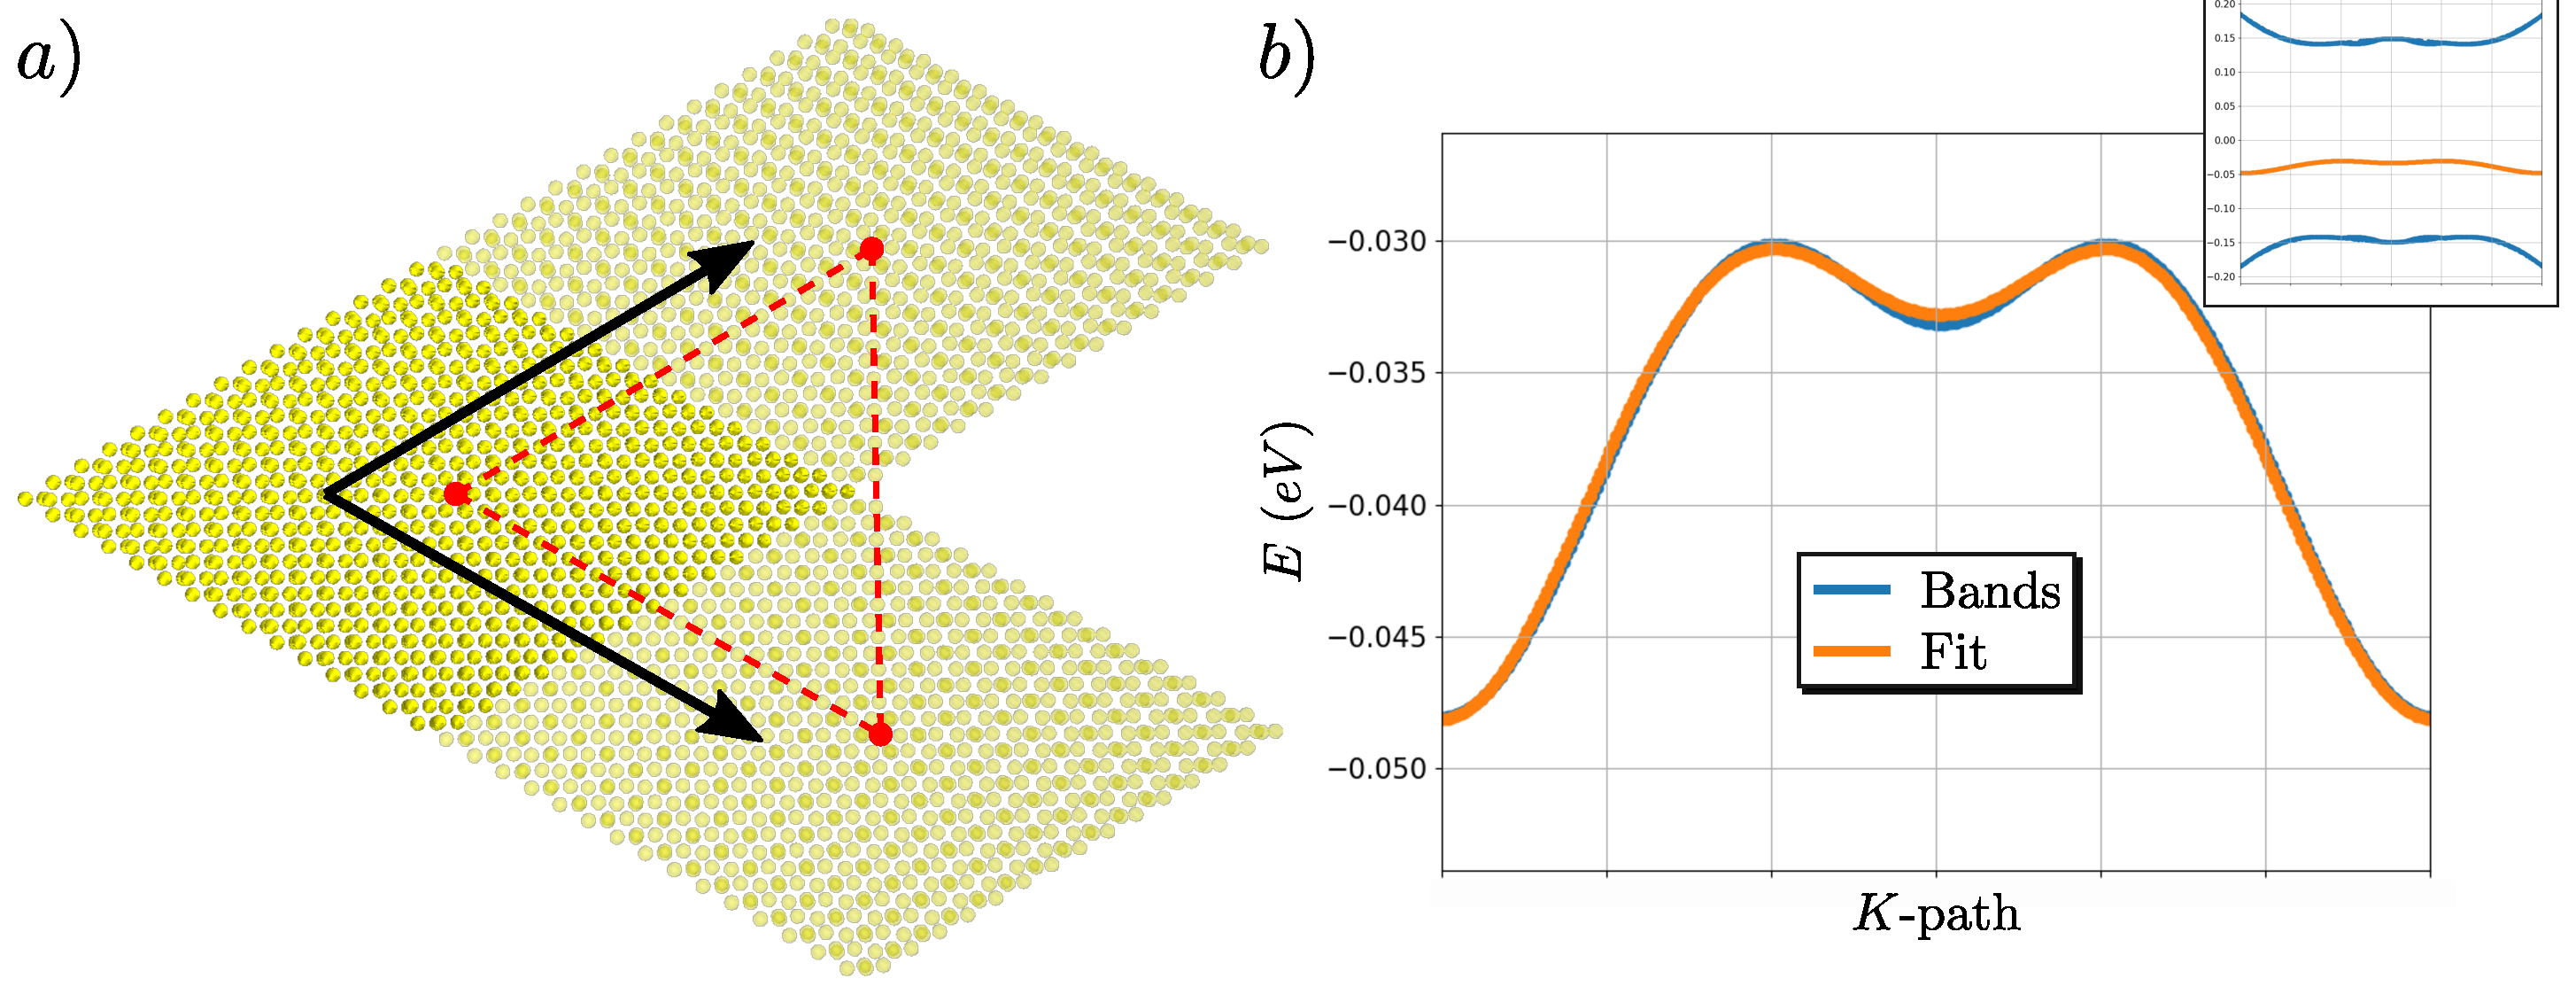
\includegraphics[width=0.8\textwidth]{artlat/fig/triangular_bands.pdf}
  \vspace{-5pt}
  \caption{$a)$ shows an example of a unit cell with the vacancies placed in such a way that the translational symmetry creates an artificial triangular lattice. $b)$ shows the in-gap bands (orange in the inset) that appear because of the vacancies, the fit is done using a model with up to third neighbors.}
  \label{triangular}
\end{figure}
\FloatBarrier
%~~~~~~~~~~~~~~~~~~~~~~~~~~~~~~~~~~~~~~~~~~~~~~~~~~~~~~~~~~~%

In Fig.~\ref{triangular} $a)$ we can be the architecture considered, a single vacancy in the center of the unit cell and the standard lattice vectors for a graphene supercell. The lattice of impurities form an in-gap band which resembles that of a triangular lattice.
In particular it can be fit to a model like:
\begin{equation}
\begin{split}
  H(k) = E_0 &+
         2t_1\left[ cos\left(\vec{k}\vec{a}_1\right) +
                    cos\left(\vec{k}\vec{a}_2\right) +
                    cos\left(\vec{k}(\vec{a}_1-\vec{a}_2)\right)
              \right] +\\
         &+2t_2\left[ cos\left(\vec{k}(\vec{a}_1+\vec{a}_2)\right) +
                    cos\left(\vec{k}(2\vec{a}_1-\vec{a}_2)\right) +
                    cos\left(\vec{k}(-\vec{a}_1+2\vec{a}_2)\right)
             \right] +\\
         &+2t_3\left[ cos\left(2\vec{k}\vec{a}_1\right) +
                    cos\left(2\vec{k}\vec{a}_2\right) +
                    cos\left(2\vec{k}(\vec{a}_1-\vec{a}_2)\right)
              \right]
\end{split}
\label{triangular_hamil}
\end{equation}
Where $\vec{k}$, $\vec{a}_1$ and $\vec{a}_2$ are the Bloch vector and the lattice vectors respectively. The parameters that best fit the model \eqref{triangular_hamil} are the following:
\begin{equation}
\begin{split}
  E_0 &= \SI{-0.036}{\eV}\\
  t_1 = \SI{-1.93e-3}{\eV} \quad;\quad
  t_2 &= \SI{7.40e-5}{\eV} \quad;\quad
  t_3 = \SI{-5.26e-5}{\eV}
\end{split}
\end{equation}


\subsection{Artificial graphene}
In order to create an artificial graphene crystal we need to place the vacancies at a particular distance that depends on the size of the chosen unit cell.
The basic unit cell and lattice vectors for graphene are
\begin{equation}
\begin{split}
  r_0 = a\left(-\frac{1}{2},0,0\right) \qquad ; \qquad
  r_1 = a\left(\frac{1}{2},0,0\right)\\
  a_1 = a\left(\frac{3}{2},\frac{\sqrt{3}}{2},0\right) \qquad ; \qquad
  a_2 = a\left(\frac{3}{2},-\frac{\sqrt{3}}{2},0\right)
\end{split}
\end{equation}
In order to separate the vacancies, bigger cells must be used, the lattice vectors will escalate for a cell of size $n$:
\begin{equation}
  \vec{a}^n_1 = n \vec{a}_1 \qquad ; \qquad \vec{a}^n_2 = n \vec{a}_2
\end{equation}
Since the vacancies have to be in the same sublattice, the possible distances for them are $d_v = 3na$, being $a=\SI{1.4}{\angstrom}$ the $C$-$C$ distance. The corresponding lattice vectors should be:
\begin{equation}
  \vec{a}^n_1 = 3na\left(\frac{3}{2},\frac{\sqrt{3}}{2},0\right) \qquad ; \qquad
  \vec{a}^n_2 = 3na\left(\frac{3}{2},-\frac{\sqrt{3}}{2},0\right)
\end{equation}
This simple relation shows that only supercells which are a multiple of 3 are feasible.


% Therefore a perfect graphene lattice will only emerge when $|\vec{a}^n_1|=|\vec{a}^n_2|=3na$. Notice that $m$ and $n$ are independent indices.
% \begin{equation}
%   |\vec{a}^n| = \sqrt{3}na \quad\Rightarrow n = \sqrt{3}m
% \end{equation}
% \red{Impossible?!}

When the vacancies are placed at that distance, and are properly oriented (see Fig~\ref{graphene}) the in-gap states interact among them forming two dispersing bands all over the Brillouin zone.
%~~~~~~~~~~~~~~~~~~~~~~~~~~ FIGURE ~~~~~~~~~~~~~~~~~~~~~~~~~%
\begin{figure}[h!]
  \centering
  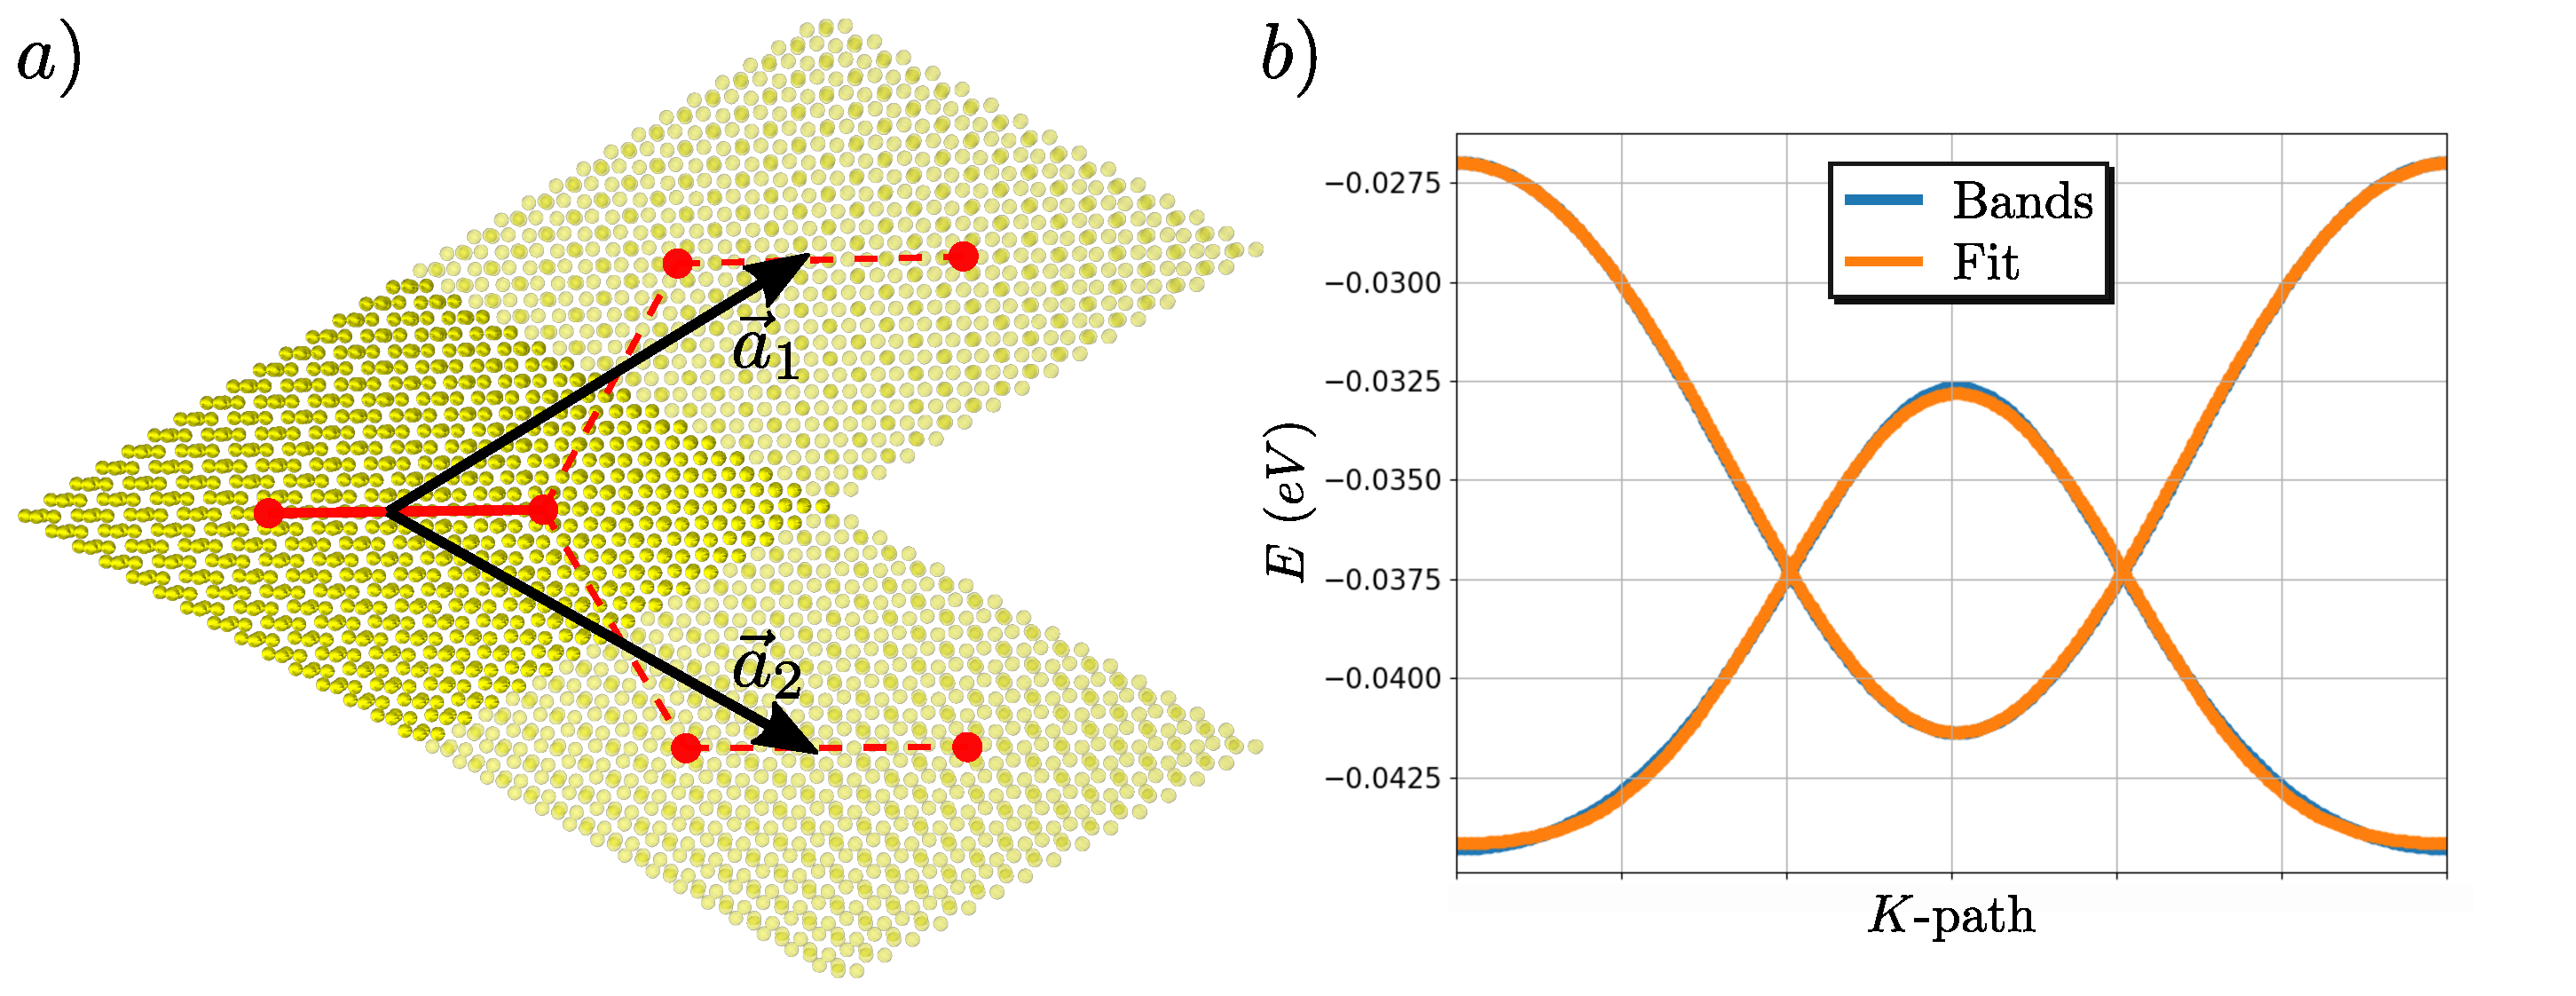
\includegraphics[width=0.8\textwidth]{artlat/fig/graphene_bands.pdf}
  \vspace{-5pt}
  \caption{$a)$ shows an example of a unit cell with the vacancies placed in such a way that the translational symmetry creates an artificial graphene lattice. $b)$ shows the in-gap bands (orange) that appear because of the vacancies, the fit is done using a model with up to third neighbors.}
  \label{graphene}
\end{figure}
\FloatBarrier
%~~~~~~~~~~~~~~~~~~~~~~~~~~~~~~~~~~~~~~~~~~~~~~~~~~~~~~~~~~~%
In Fig.~\ref{graphene} $b)$ we can see the dispersing in-gap bands as well as a fit of said bands to a simple model with up to third neighbors.

\begin{equation}
\begin{split}
  % E_0 = \SI{-0.03670772697798405}{\eV}
  % t_1 = \SI{-0.003216525825060562}{\eV}
  % t_2 = \SI{0.00018838793316003813}{\eV}
  % t_3 = \SI{0.0003533798537212944}{\eV}
  E_0 &= \SI{-0.037}{\eV}\\
  t_1 = \SI{-3.22e-3}{\eV} \quad;\quad
  t_2 &= \SI{1.88e-4}{\eV} \quad;\quad
  t_3 = \SI{3.53e-4}{\eV}
\end{split}
\end{equation}

%~~~~~~~~~~~~~~~~~~~~~~~~~~ FIGURE ~~~~~~~~~~~~~~~~~~~~~~~~~%
\begin{figure}[!ht!]
\centering
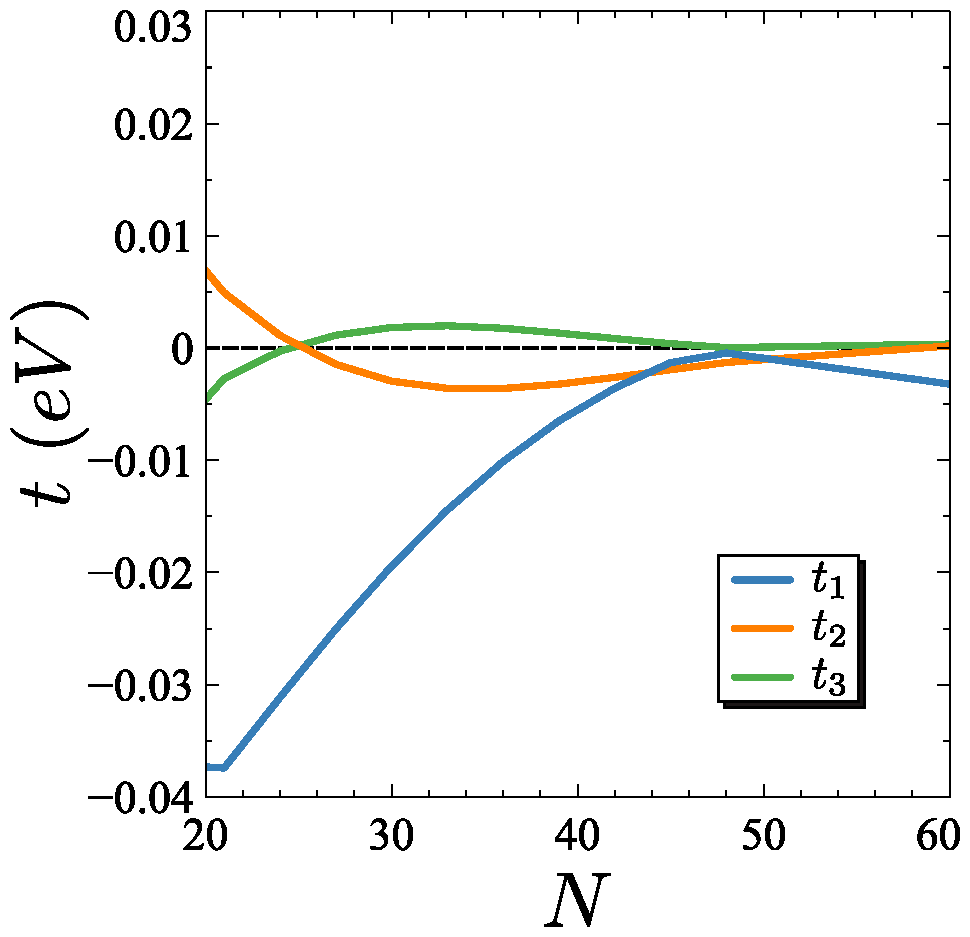
\includegraphics[width=0.5\textwidth]{artlat/fig/params.pdf}
\vspace{-5pt}
\caption{Evolution of the hopping parameters of a graphene tight-binding model with third neighbor hoppings.}
\label{hopp}
\end{figure}
\FloatBarrier
%~~~~~~~~~~~~~~~~~~~~~~~~~~~~~~~~~~~~~~~~~~~~~~~~~~~~~~~~~~~%






\subsection{Artificial Kagome}
the position of the adatoms to have an artificial Kagome lattice are:
\begin{equation}
  r_1 = \frac{a_k}{2}\left(\sqrt{3}/2,  0 ,0\right),\quad
  r_2 = \frac{a_k}{2}\left(-\sqrt{3}/2,1,0\right),\quad
  r_3 = \frac{a_k}{2}\left(-\sqrt{3}/2,-1,0\right)
\end{equation}

where $a_k = |a_1|/2$. This geometry only works regularly for odd supercells as seeing in Fig.~\ref{kagome}


%~~~~~~~~~~~~~~~~~~~~~~~~~~ FIGURE ~~~~~~~~~~~~~~~~~~~~~~~~~%
\begin{figure}[h!]
  \centering
  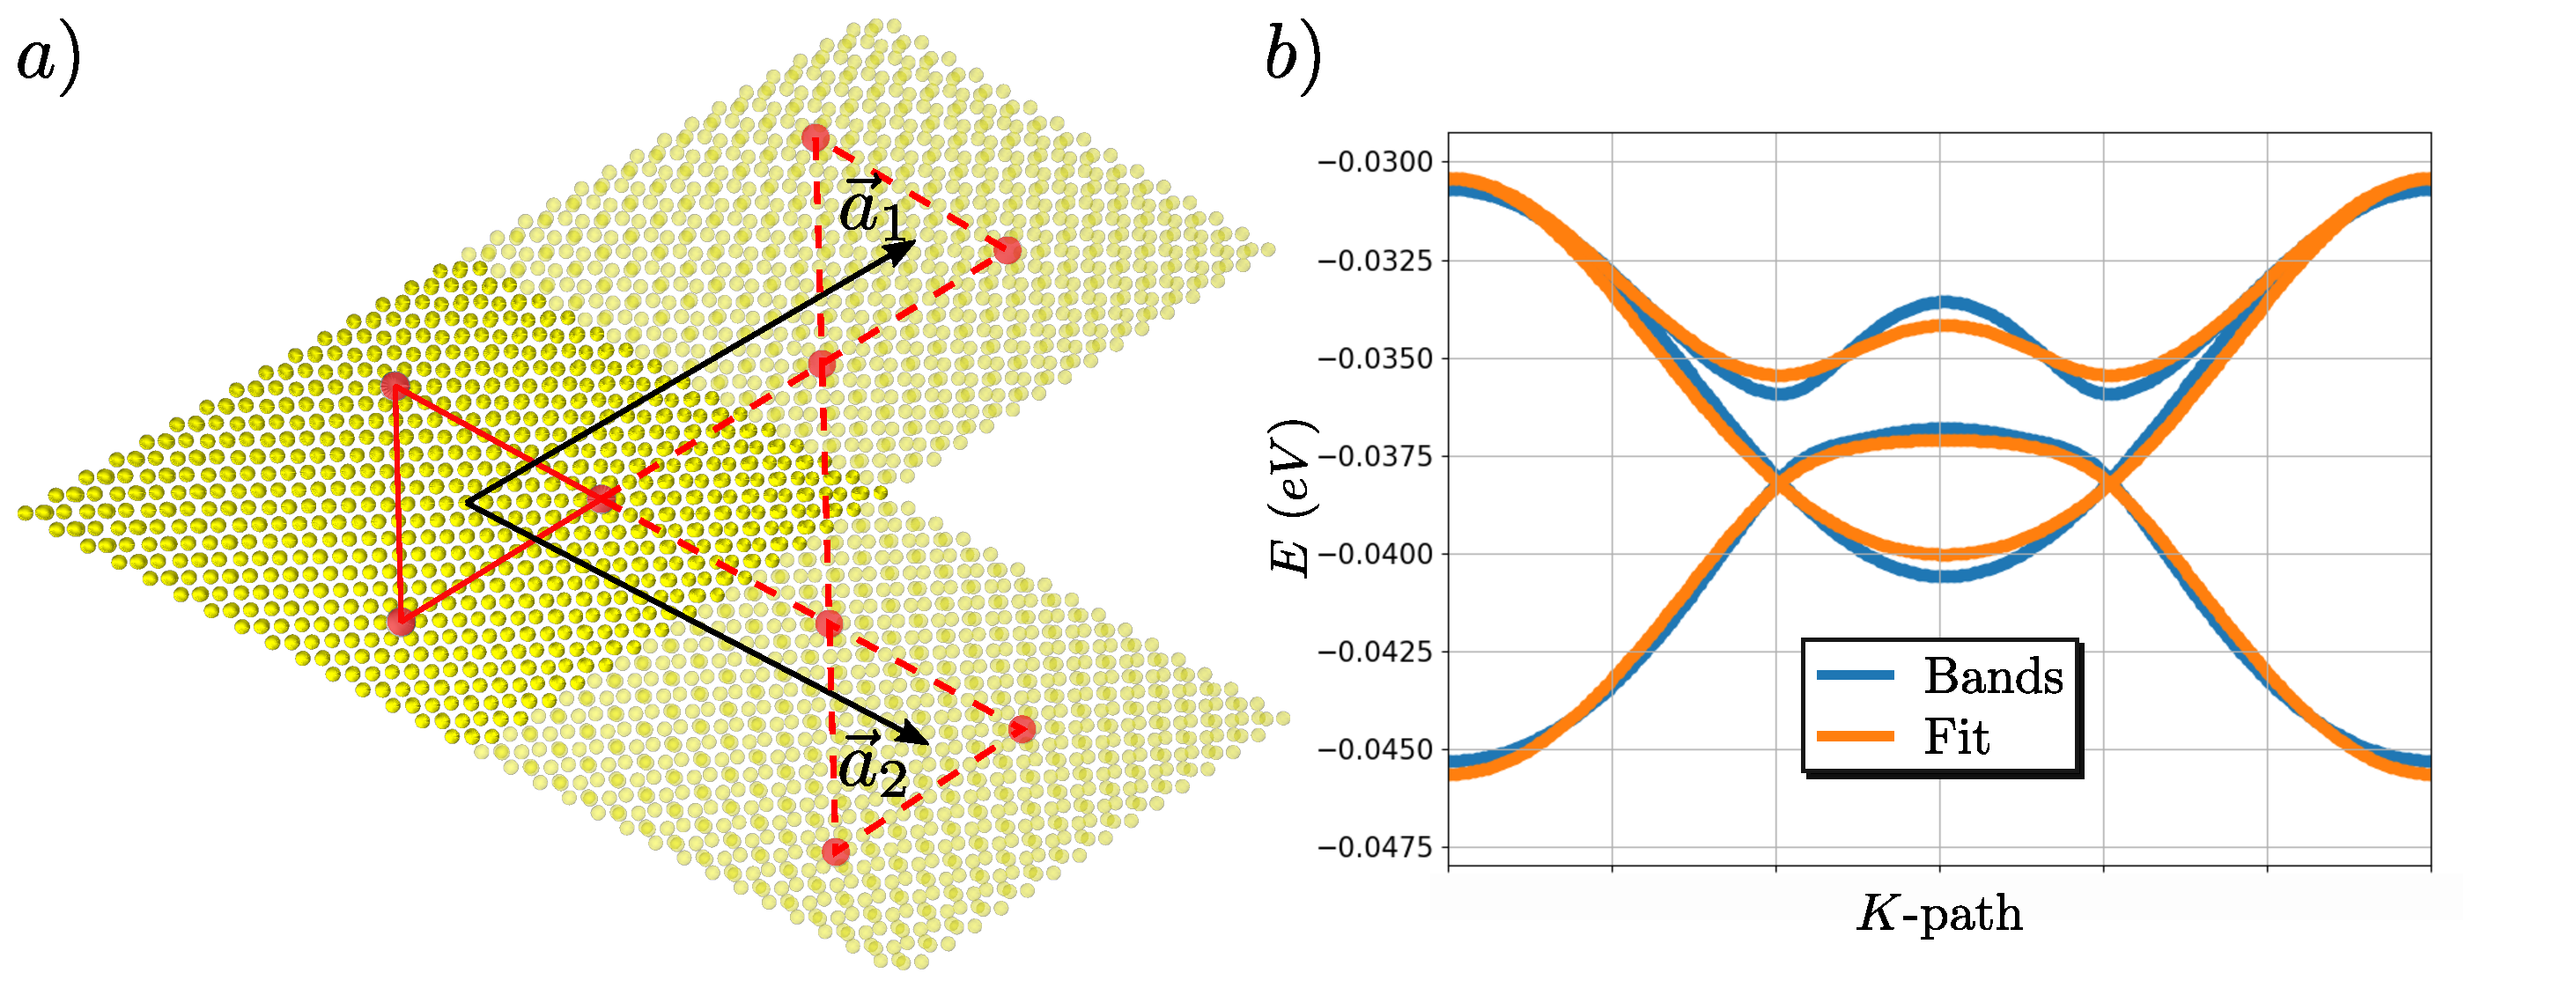
\includegraphics[width=0.8\textwidth]{artlat/fig/kagome_bands.pdf}
  \vspace{-5pt}
  \caption{$a)$ shows an example of a unit cell with the vacancies placed in such a way that the translational symmetry creates an artificial Kagome lattice. $b)$ shows the in-gap bands (orange) that appear because of the vacancies, the fit is done using a model with up to second neighbors.}
  \label{kagome}
\end{figure}
\FloatBarrier
%~~~~~~~~~~~~~~~~~~~~~~~~~~~~~~~~~~~~~~~~~~~~~~~~~~~~~~~~~~~%
\begin{equation}
\begin{split}
  % E_0 = -0.03669201703555982
  % t_1 = -0.002000033597883536
  % t_2 = -0.000536649553068988
  % t_3 = 0.00020143407845221853
  E_0 &= \SI{-0.037}{\eV}\\
  t_1 = \SI{-2.00e-3}{\eV} \quad;\quad
  t_2 &= \SI{-5.37e-4}{\eV} \quad;\quad
  t_3 = \SI{2.01e-4}{\eV}
\end{split}
\end{equation}
A geometric cheat sheet can be found in appendix~\ref{models}





\section{Parameters control. Hubbard dimer}

In order to determine the ground state as a function of both the electric field $\mathcal{E}$ and the distance between vacancies $d$ we use the fact that the spectrum of the blue Hamiltonian looks like one of the structures shown in Fig.~\ref{spectrum_dimer}. Considering the standard deviation of the 3 lowest eigenvalues (0-2), and the same quantity skipping one eigenvalue (1-3) we can obtain a quantity that will flip sign if the singlet and triplet cross.

%~~~~~~~~~~~~~~~~~~~~~~~~~~ FIGURE ~~~~~~~~~~~~~~~~~~~~~~~~~%
\begin{figure}[h!]
\centering
  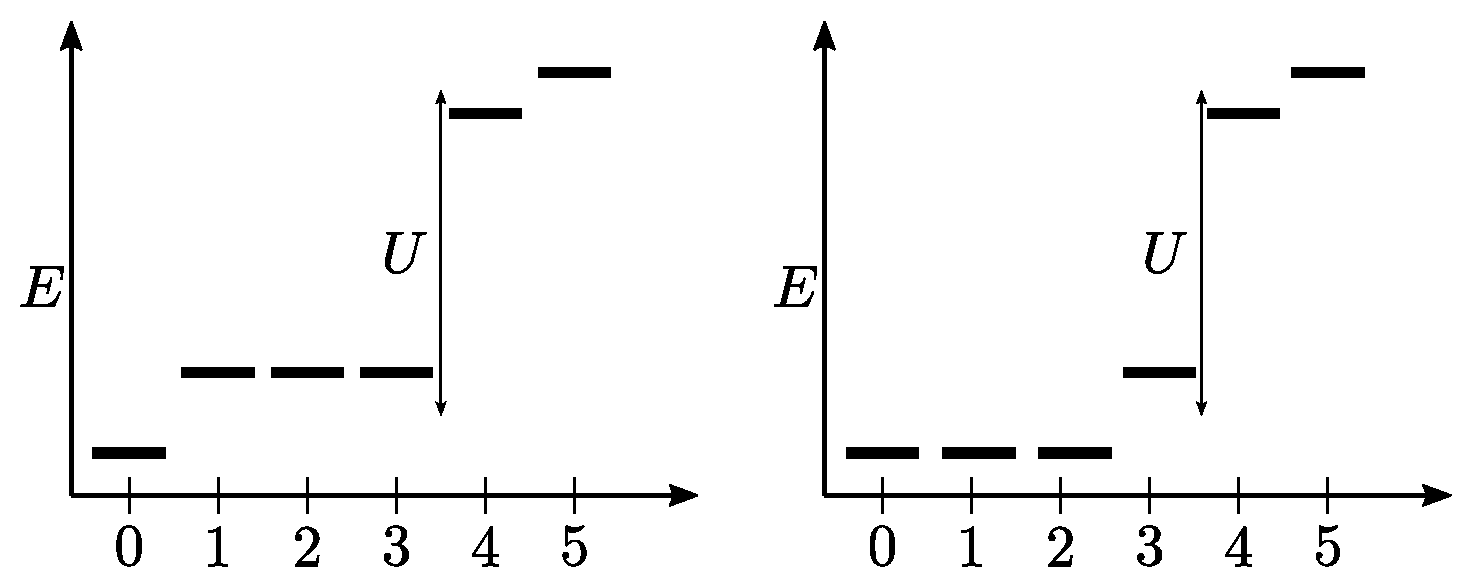
\includegraphics[width=0.7\textwidth]{artlat/fig/sketch_levels.pdf}
\vspace{-5pt}
\caption{Possible structure of the spectrum of the eigenvalues of the blue Hamiltonian.}
\label{spectrum_dimer}
\end{figure}
\FloatBarrier
%~~~~~~~~~~~~~~~~~~~~~~~~~~~~~~~~~~~~~~~~~~~~~~~~~~~~~~~~~~~%

%~~~~~~~~~~~~~~~~~~~~~~~~~~ FIGURE ~~~~~~~~~~~~~~~~~~~~~~~~~%
\begin{figure}[h!]
\centering
  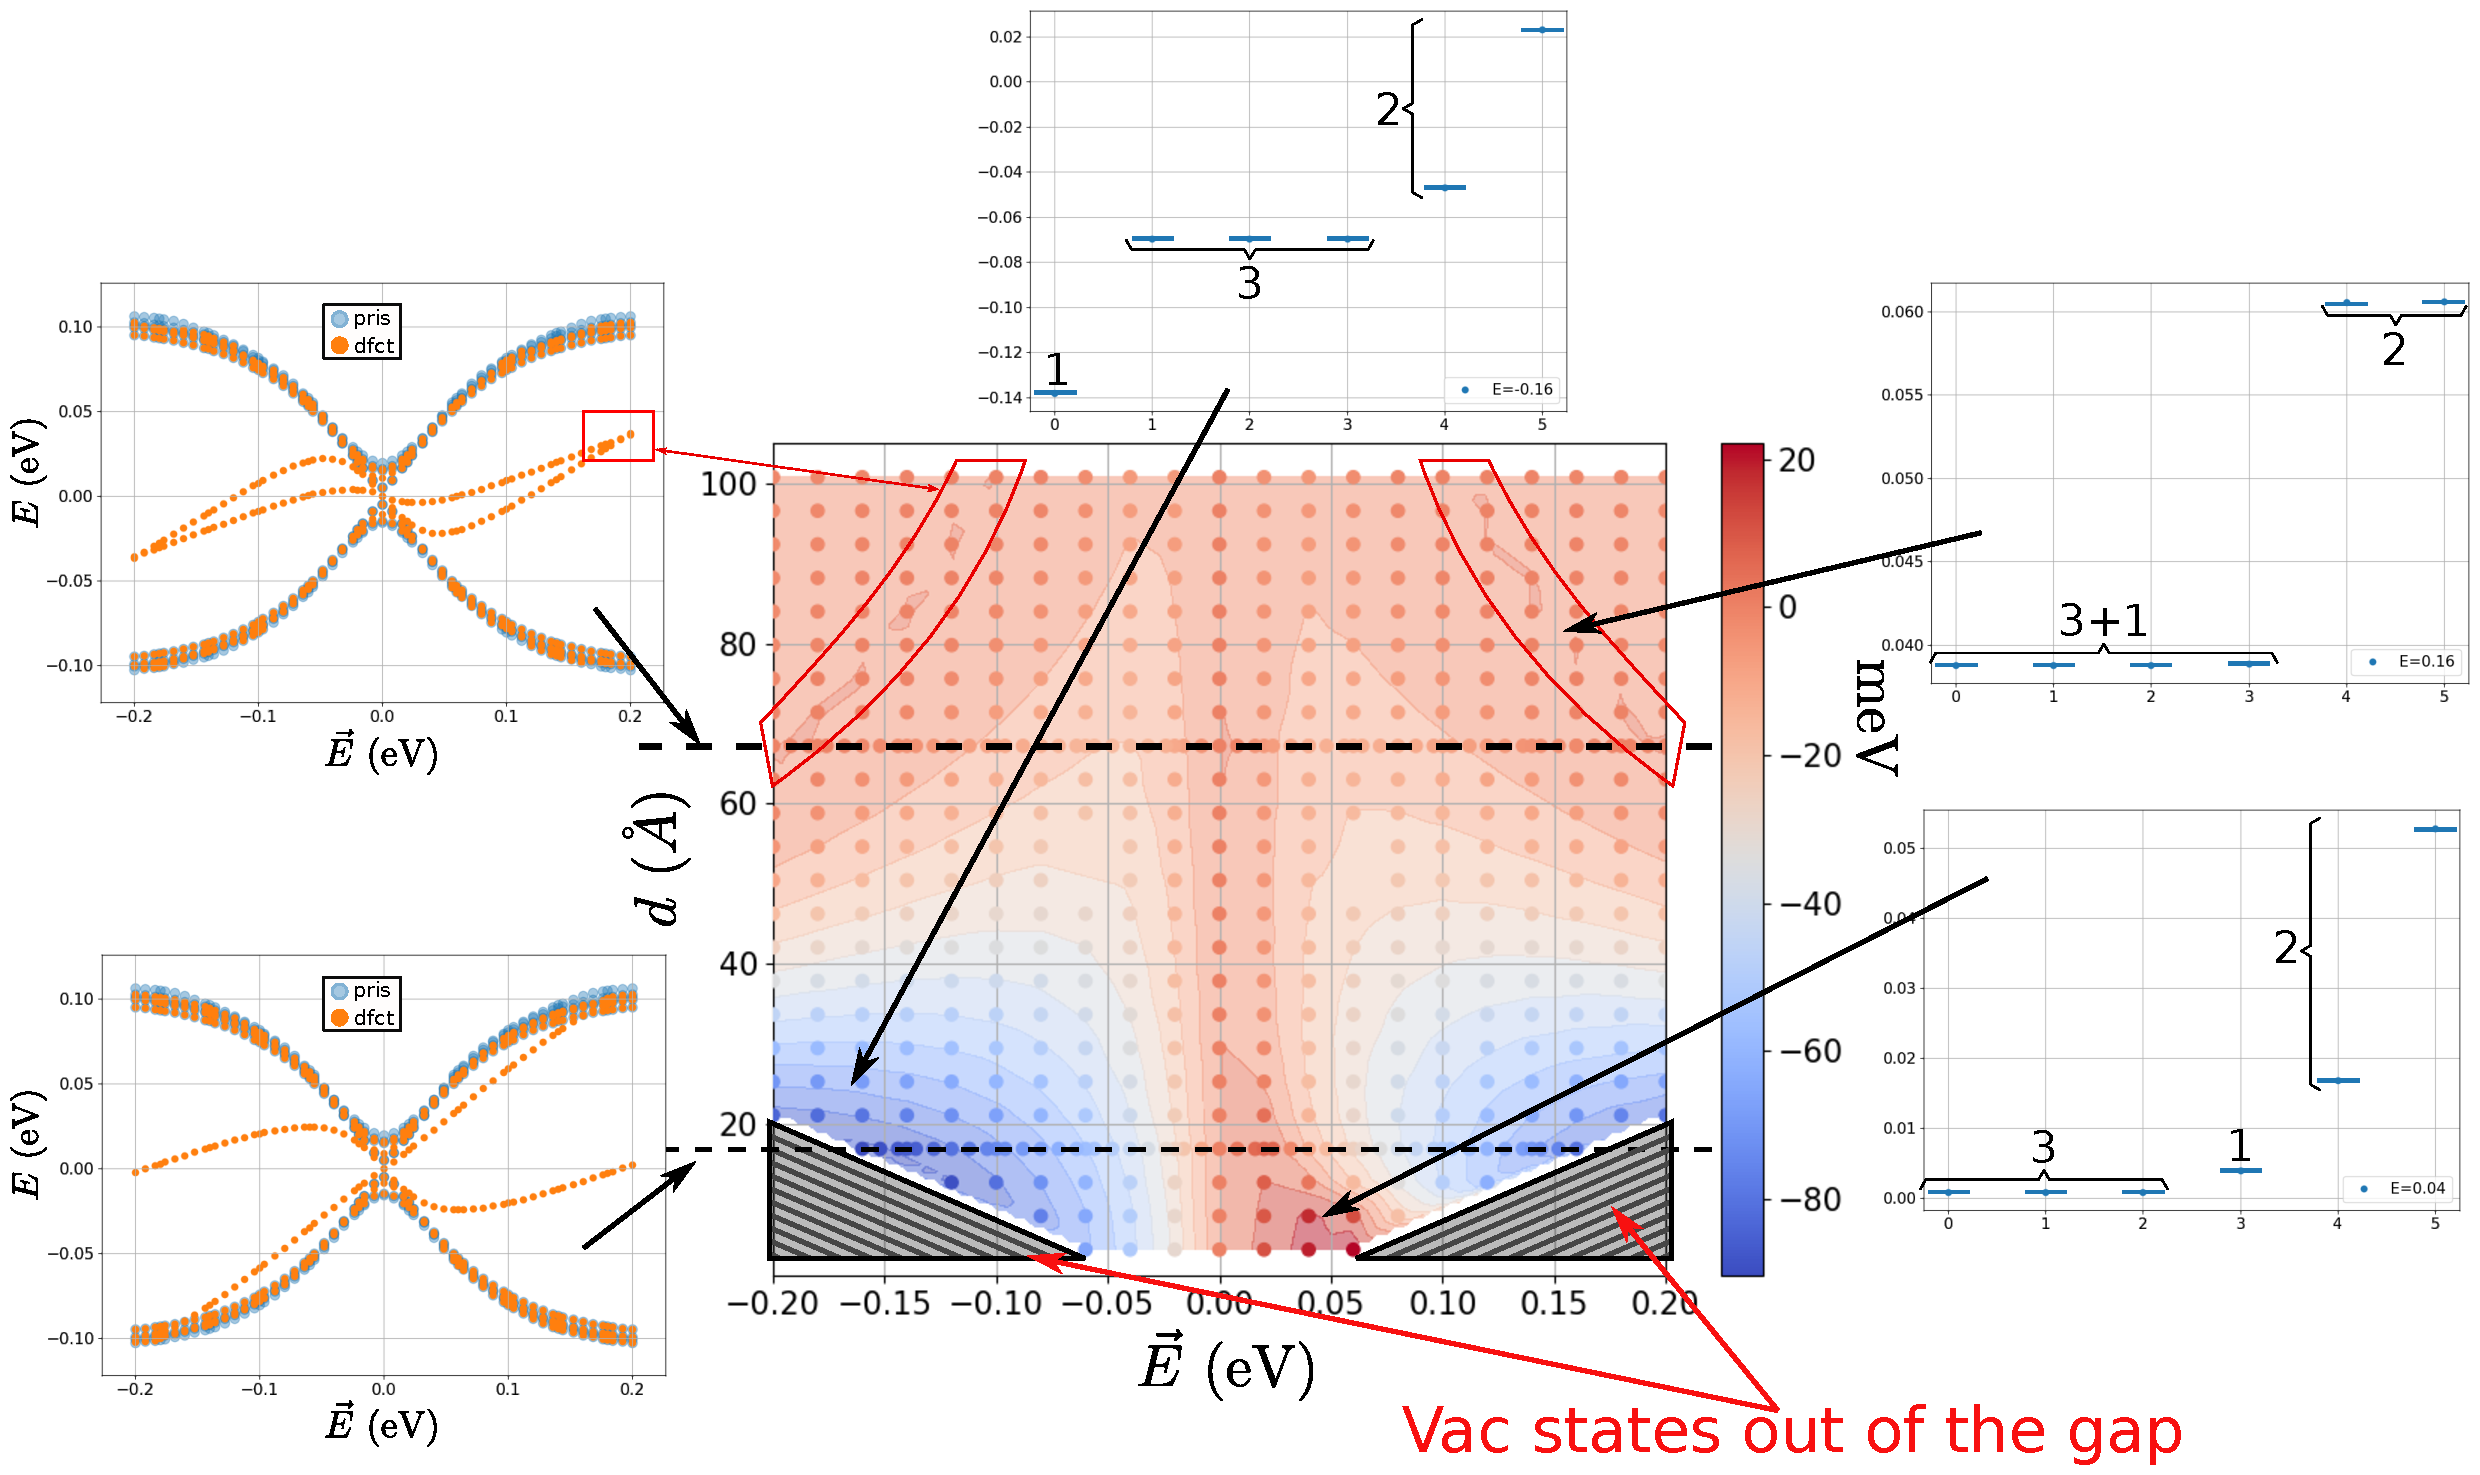
\includegraphics[width=0.7\textwidth]{artlat/fig/phase_J.pdf}
\vspace{-5pt}
\caption{Phase space showing the arrangement of the ground state as exposed in the text}
\label{}
\end{figure}
\FloatBarrier
%~~~~~~~~~~~~~~~~~~~~~~~~~~~~~~~~~~~~~~~~~~~~~~~~~~~~~~~~~~~%

%~~~~~~~~~~~~~~~~~~~~~~~~~~ FIGURE ~~~~~~~~~~~~~~~~~~~~~~~~~%
\begin{figure}[h!]
\centering
  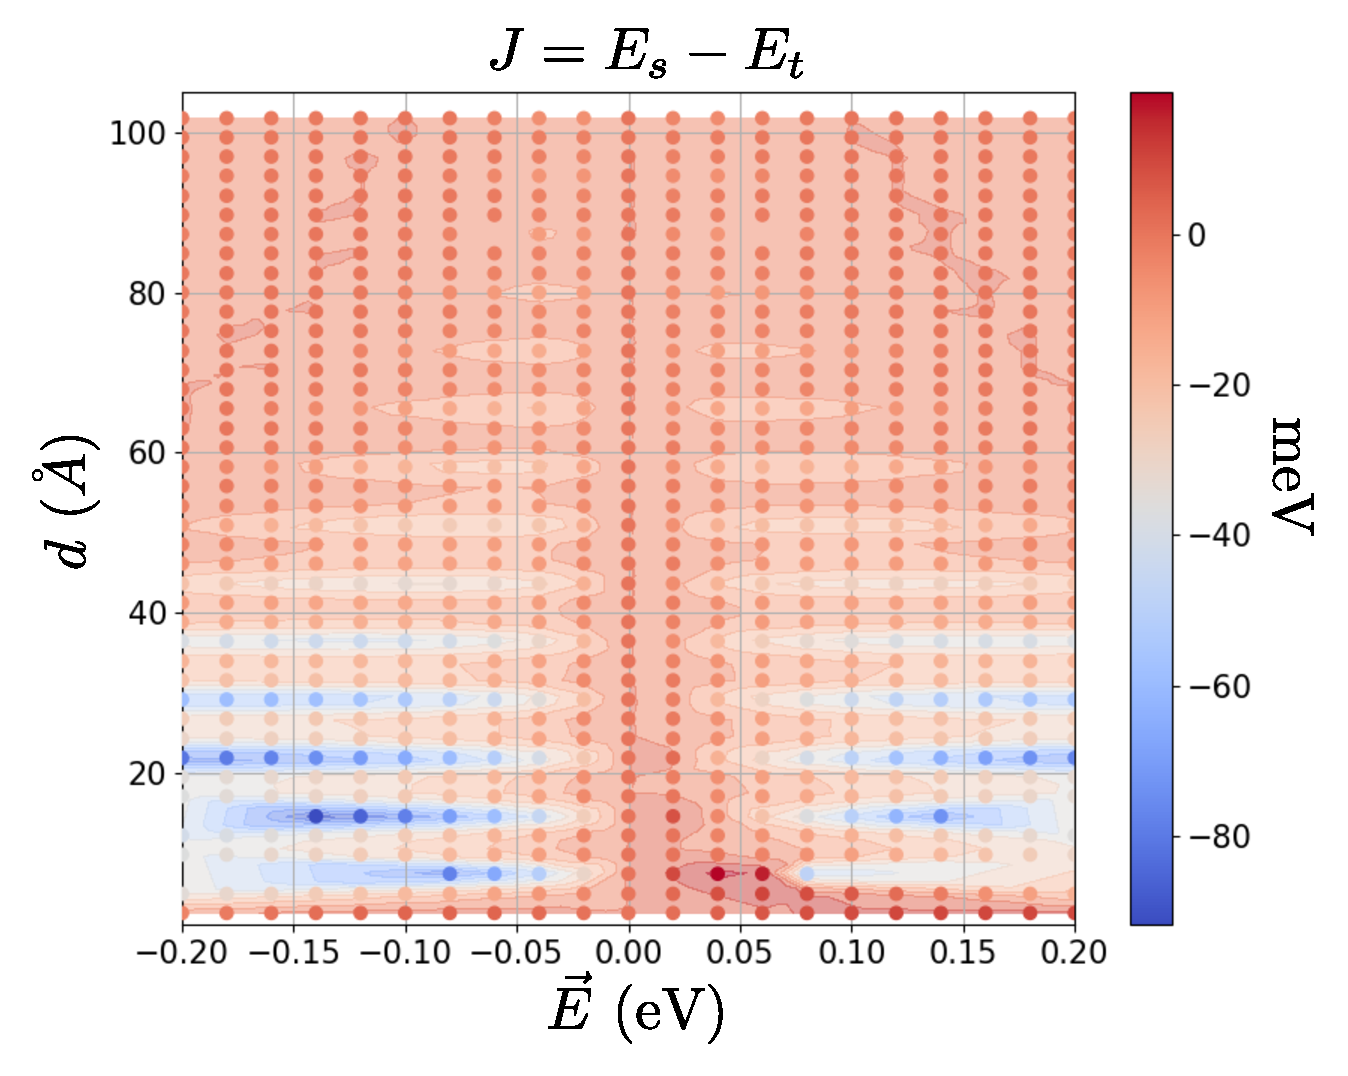
\includegraphics[width=0.7\textwidth]{artlat/fig/phase_J30.pdf}
\vspace{-5pt}
\caption{Phase space showing the arrangement of the ground state as exposed in the text for $\alpha=30$}
\label{}
\end{figure}
\FloatBarrier
%~~~~~~~~~~~~~~~~~~~~~~~~~~~~~~~~~~~~~~~~~~~~~~~~~~~~~~~~~~~%

